
\chapter{Optimisation}
\epigraph{Relax. As usual, I will bore you with the details.}%
{\textsc{---chris lee}}

The previous chapter discussed the architecture of the Accelerate language
embedding and execution on CUDA hardware. Through a set of benchmarks, we
identify the two most pressing performance limitations: operator fusion and data
sharing. This chapter describes the method used to overcome these issues,
focusing primarily on the approach to operator fusion in the context of the
stratified Accelerate language and skeleton-based implementation of the CUDA
backend.

It should be noted that ``optimisation'' is a misnomer; only rarely does
applying optimisations to a program result in object code whose performance is
optimal, by any measure. Rather, the goal is to \emph{improve} the performance
of the object code generated by a backend, although it is entirely possible that
they may decrease it or make no difference at all. As with many interesting
problems in [computer] science, in most cases it is formally undecidable whether
a particular optimisation improves, or at least does not worsen, performance.

In general, we would like to be as aggressive as possible in improving code, but
not at the expense of making it incorrect.


\section{Redundancy Elimination}
\label{sec:redundancy_elimination}

The optimisations in this section deal with the elimination of redundant
computations. These procedures almost always improve the performance of the code
they are applied to.

\subsection{Sharing Observation}

As described in section~TK, operations of the embedded language do not
directly issue computations; instead, they build \emph{abstract syntax
trees}\index{abstract syntax tree}\index{AST|see{abstract syntax tree}} that
represent the embedded computation. These term trees use \indexe{higher-order
abstract syntax} (HOAS)\index{higher-order abstract syntax} to embed
function-valued scalar expressions as well as typeclass overloading to reflect
arithmetic expressions.

A well known problem of defining (deeply) embedded languages in this way is that
a straightforward reification of the surface language program would result in a
complete unfolding of the expression into embedded language terms. That is, each
occurrence of a let-bound variable in the source program would create a separate
unfolding of the bound expression in the compiled code. For example, consider
the following program:
%
\begin{lstlisting}[style=Haskell]
let ys = map f xs
in  zipWith g ys ys
\end{lstlisting}
%
If we do not take care, the expression will be inefficiently translated as:
%
\begin{lstlisting}[style=Haskell]
zipWith g (map f xs) (map f xs)
\end{lstlisting}

This problem was solved elegantly by \citet{Gill:2009dx} who proposed the use
of \index{stable name}\emph{stable names}~\cite{PeytonJones:2000ks} to recover
sharing of source terms in a deeply embedded language. Unfortunately, Gill's
original approach (1) reifies the abstract syntax in \emph{graph} form, and (2)
assumes an \emph{untyped} syntax representation. We use a variant of Gill's
technique that instead preserves types and produces a tree with minimal
flattening~\cite{McDonell:2013wi}, which is able to recover exactly those let
bindings used in the source program.

The higher-order abstract syntax\index{higher-order abstract syntax}
representation of the surface language, while convenient for the human reader,
is awkward for program transformations as it complicates looking under lambdas.
We convert the source representation to a type-safe internal representation
based on nameless \indext{de Bruijn} indices in the style of
\citet{Altenkirch:2003kz}, using GADTs \cite{Jones:2006eh} and type families
\cite{Chakravarty:2005dx,Schrijvers:2008ir} to preserve the embedded program's
type information. While developed independently
\cite{McDonell:2013wi,Chakravarty:2009uo}, this conversion is similar to the
\emph{unembedding} of \citet{Atkey:2009dj}. Unembedding and sharing recovery are
necessarily intertwined. Sharing recovery must be performed on the source
representation, otherwise sharing will have already been lost, but we can not
perform sharing recovery on higher-order abstract syntax\index{higher-order
abstract syntax} as we need to traverse below the lambda abstractions. Hence,
both operations go hand in hand. In brief the method proceeds in three stages:


\paragraph{Phase 1: Prune shared terms:}

A top-down traversal of the AST\index{abstract syntax tree} annotates each node
with its unique stable name\index{stable name}, and builds an occurrence map for
the number of times we see each node in the overall program. The stable names of
two Haskell terms are equal only when the terms are represented by the same heap
structure in memory. Likewise, when the abstract syntax tree of two terms of an
embedded language program have the same stable name, we know that they represent
the same value. If we encounter a node already in the occurrence map, it represents a
previously visited node and is thus a \emph{shared subterm}. We replace the
entire subterm at that node with a placeholder containing its stable name. In
this way all but the first occurrence of a shared subterm are pruned and
replaced with variable bindings, so that we do not descend into terms that have
been previously encountered. This avoids completely unfolding the embedded
expression, so the complexity of sharing observation is proportional to the
number of nodes in the tree \emph{with} sharing.

As the stable name of an expression is an intensional property, it can only be
determined in Haskell's \code{IO} monad, and strictly speaking because of this
it is not deterministic. The stable name API does not guarantee completeness:
for two stable names \code{sn1} and \code{sn2}, if \code{sn1 == sn2} then the
two stable names were created from the same heap object. However, the reverse is
not necessarily true; if the two stable names are not equal the objects they
come from may still be equal. Put another way, equality on stable names may
return a false negative, which means that we fail to discover some sharing, but
can never return a false positive since stable names from different heap objects
are not considered equal. Luckily, sharing does not affect the denotational
meaning of the program, and hence a lack of sharing does not compromise
denotational correctness.


\paragraph{Phase 2: Float shared terms:}

A bottom-up traversal that determines the scope for every binding to be
introduced to share a subterm. It uses the occurrence map to determine, for
every shared subterm, the meet of all the shared subterm occurrences --- the
lowest AST node at which the binding for the subterm can be placed. This is why
the occurrence map generated in the previous phase can not be simplified to
a set of occurring names: we need the actual occurrence count to determine where
shared subterms should be let-bound.


\paragraph{Phase 3: Binder introduction:}

Finally, each floated subterm gets let-bound right above the node it floated to.
At the same time, we convert the AST into nameless \indext{de Bruijn} form by
introducing de Bruijn indices at the same time as introducing the lets.\\


\subsection{Common Subexpression Elimination}
\label{sec:cse}

\emph{Common subexpression elimination} finds computations that are performed at
least twice on a given execution path and eliminates the second and later
occurrences, replacing them with uses of saved values. The current
implementation performs a simplified version of common subexpression
elimination, where we look for expressions of the form:
%
\begin{lstlisting}[style=Haskell,numbers=none]
%\bf$\langle$ common subexpression elimination $\rangle$% let x = e1 in [x/e1]e2
\end{lstlisting}
%
and replace all occurrences of \code{e1} in \code{e2} with \code{x}. This might
not completely eliminate redundant expressions from the program, as it will not
eliminate any common subterms not already defined in the source program. It will
however catch some cases, in particular those that tend to be introduced during
the array fusion optimisation.
%\footnote{\url{http://hackage.haskell.org/trac/ghc/ticket/701}}

While it may seem that common subexpression elimination is always worthwhile, as
it reduces the number of arithmetic operations performed, this is not
necessarily advantageous. The simplest case in which it may not be desirable is
if it causes a register to be occupied for a long time in order to hold the
shared expression's value, which hence reduces the number of registers available
for other uses. Even worse is if that value has to be spilled to memory because
there are insufficient registers available. We sidestep this tricky and
target-dependent issue by, for now, simply ignoring it.



\section{Array Fusion}
\label{sec:fusion}

Fusion, or deforestation, is a term used to describe techniques for having a
compiler automatically eliminate intermediate data structures in a computation
by combining successive traversals over these structures. For example, to
compute the sum of squares of all integers from one to a given number in
Haskell~\cite{Haskell:1998}, I could write:
%
\begin{lstlisting}[style=haskell]
sum_of_squares :: Int -> Int
sum_of_squares n
    = sum                       -- add all numbers in the list
    $ map (\x -> x * x)         -- traverse list doubling each element
    $ enumFromTo 1 n            -- generate list of numbers [1..n]
\end{lstlisting}
%
but while the meaning of the program is clear, it is inefficient, as this code
produces two intermediate lists of numbers which each require $O(n)$ memory to
store and data transfers to manipulate. Instead, one could write the program
as a single tail-recursive loop as such:
%
\begin{lstlisting}[style=haskell]
sum_of_squares :: Int -> Int
sum_of_squares n = go 1 0
  where
    go i acc | i > n     = acc                   -- return final tally
             | otherwise = go (i+1) (acc + i*i)  -- add to accumulator and step to next element
\end{lstlisting}
%
The second program is much more efficient than the first because it does not
involve the production of any intermediate lists and executes is constant space.
Unfortunately, the clarity of the original program has been lost. What we
\emph{really} want is to write the first program, and have the compiler
\emph{automatically} transform it into the second, or something morally
equivalent.

This example also demonstrates a subtle behavioural tendency of optimising
program transformations: while the second (target) program does not produce any
intermediate data structures as desired, we can no longer interpret the program
as a sequence of combinators. This observation is critical if the combinators
represent \emph{collective} operations as they do in Accelerate: while the
second program compiles to an efficient scalar loop, its \emph{parallel}
interpretation has been lost.


\subsection{Related Work}
\label{sec:fusion_related_work}

The desire to program in a functional style while still achieving the
performance level of an imperative language has been around for as long as
functional programming itself. Fusion has received plenty of attention in the
context of functional program. This section briefly summarises some of the key
milestones in the history of deforestation as a compiler optimisation that
influences this work.

\subsubsection{Deforestation}

% blugh blurgh
Inspired by earlier work in \code{fold/unfold} methods (for example
\citet{Burstall:1977kl}), Philip Wadler set out to develop a technique that
would \emph{automatically} remove intermediate structures from functional
programs, a technique he (later) dubbed \indexe{deforestation}
\cite{Wadler:1981hy,Wadler:1990ix}.

The method identifies a core set of list operators that can be used to express a
large class of computations: \code{map}, \code{reduce} and \code{generate} (the
latter being similar in spirit to \code{foldr} and \code{unfoldr} respectively),
together with a collection of rewrite rules that apply to combinations of these
operators. These rules identify specific patterns of list operators that create
then consume intermediate lists, then merges these operations to avoid the
intermediary.

\paragraph{Advantages}
\begin{itemize}
    \item Automatic: does not require programmer input, and therefore suitable
        for integration to a compiler.

    \item Source-to-source: all transformations take valid programs in the
        source language and output (faster) valid programs in the source
        language. This makes the output of deforestation easy to integrate as
        part of a compiler pipeline.

    \item Simple: each rule is easy to understand and obviously correct.
\end{itemize}

\paragraph{Disadvantages}
\begin{itemize}
    \item Each optimisation requires a separate transformation rule. If we want
        to add new list operators, we need to add a new rule for each
        combination of the new operator with each existing operator. This does
        not scale.

    \item Limited: many computations can not be expressed in terms of these
        three operations, so the framework can not eliminate intermediate lists
        in these case.
\end{itemize}


\subsubsection{foldr/build}

Building upon the original deforestation algorithm, Andy Gill's doctoral thesis
introduces another approach to deforestation known as \emph{foldr/build
fusion}~\cite{Gill:1996tf,Gill:1993de}.
\index{fusion!foldr/build}\index{foldr/build|see{fusion!foldr/build}}
% This techniques performs a range of optimisations as broad as previous
% approaches the listless transformer \cite{Wadler:1984ia,Wadler:2005iw} while
% addressing their drawbacks.
Like the deforestation algorithm, \code{foldr/build} fusion is a rule-based
source-to-source transformation. In fact, it is based on a single rule:
%
\begin{lstlisting}[style=Haskell,numbers=none,mathescape,caption={The \code{foldr/build} transformation}]
%\bf$\langle$ foldr/build fusion $\rangle$% forall g k z. foldr k z (build g) $\mapsto$ g k z

build :: (forall b. (a -> b -> b) -> b -> b) -> [a]
foldr :: (a -> b -> b) -> b -> [a] -> b
\end{lstlisting}

The idea is to think of \code{build} as a function that constructs a list, and
\code{foldr} as a list consumer. Because of this uniform treatment of lists as
\emph{complete objects}, rather than being composed of many individual
constructor cells, we can have a single \code{foldr/build} rule analogous to
standard case reduction rules, but instead of removing a single constructor
removes the \emph{entire data structure}. This method became the first
non-trivial deforestation system to be included as an active part of a
production quality functional language compiler.

\paragraph{Advantages}
\begin{itemize}
    \item Simple, automatic, source-to-source transformation.

%    \item No limitation on inputs: \code{foldr/build} fusion operates over the
%        entire Haskell language. When a list is produced without using
%        \code{build} or consumed without using \code{foldr}, the
%        deforestation scheme is not hampered and simply leaves the list intact.

    \item Single rule: unlike the original deforestation algorithm, a single
        rule suffices. When new list operations are added, so long as they can
        be expressed in terms of \code{foldr} and \code{build}, the
        transformation will apply; there is no need to consider all combinations
        with the existing operations.
\end{itemize}

\paragraph{Disadvantages}
\begin{itemize}
    \item The transformation can not handle functions that use accumulators,
        such as \code{foldl}, or consume multiple inputs, such as
        \code{zip}.

    \item Operations that do not produce lists using \code{build} or consume
        them using \code{foldr} will not have the intermediate list
        eliminated.
\end{itemize}


\subsubsection{Stream Fusion}

Following Gill's work, a whole cottage industry of new deforestation approaches
appeared with the goal of covering the cases left out by
\code{foldr/build}\index{fusion!foldr/build}. Most of that work was
theoretical, a lot of it was based on category theory, and almost none of it had
any impact in practice. Unlike those systems of the prior two decades,
\emph{stream fusion}\index{fusion!stream}~\cite{Coutts:2007kp} succeeded in this
goal and at the same time stayed simple and useful in practice.

Stream fusion has a similar structure to \code{foldr/build}: a single rule
eliminates matching pairs of constructor and destructor, and operations need to
be expressed in terms of these constructors:
%
\begin{lstlisting}[style=Haskell,numbers=none,mathescape,caption={The \emph{stream fusion} transformation}]
%\bf$\langle$ stream fusion $\rangle$% forall s. stream (unstream s) $\mapsto$ s

stream   :: [a] -> Stream a
unstream :: Stream a -> [a]

data Stream a = exists s. Stream (s -> Step a s) s
data Step a s = Done
              | Yield a s           -- produce a value and new state
              | Skip s              -- update the state without producing a value
\end{lstlisting}

Streams have some abstract state and a \emph{stepper} function that advances the
stream from one state to the next, possibly yielding a new value. The
\code{stream} constructor \code{Yield}s values from its input until it runs
out, and the \code{unstream} destructor build a list by consuming its input
stream until encountering \code{Done}, discarding \code{Skip}s along the
way. The \code{Stream} constructors are chosen so as to keep the definition of
each element as a non-recursive function. When \code{Stream}s are fused by
applying the rule, this enables the compiler to aggressively apply standard
optimisation techniques.

\paragraph{Advantages}
\begin{itemize}
    \item Preserves the nice properties of
        \code{foldr/build}\index{fusion!foldr/build} fusion.
    \item Adds supports operations with accumulators and multiple inputs.
\end{itemize}

\paragraph{Disadvantages}
\begin{itemize}
    \item Fuses a sequence of bulk operations into a single scalar loop, losing
        the parallel interpretation of the program.
\end{itemize}



\subsubsection{Data Parallel Haskell}
\code{split/join}\index{fusion!split/join} fusion from
DPH.\index{data-parallel Haskell}\index{DPH|see{data-parallel Haskell}}
\citet{Chakravarty:2007tc,Jones:2008uu}.


\subsubsection{Delayed Arrays}

The previous fusion transformations are based on the idea of expressing
computations in terms of a builder and consumer function, and then having the
compiler identify and remove adjacent constructor/destructor pairs. In contrast,
the Repa~\cite{Keller:2010er} library uses a functional representation of
\emph{delayed arrays}\index{fusion!delayed arrays} that instead \emph{avoids}
creating unnecessary intermediate structures, rather than relying on a
subsequent fusion transformation to remove them.

\begin{lstlisting}[style=Haskell,numbers=none,caption={Repa-1 style array definition},label={lst:repa_arrays}]
data Array sh e = Manifest sh (Vector e)    -- unboxed data
                | Delayed  sh (sh -> e)     -- array shape and indexing function
\end{lstlisting}

The key principle of the design is to avoid generating an explicit
(\code{Manifest}) representation of intermediate arrays that can instead be
represented as a transformation function from array indices to values.

% Repa retains the functional programming style by exposing an interface of
% collective operations over arrays --- such as maps, folds, and permutations ---
% instead of the imperative style of reading and writing individual array
% elements.

\paragraph{Advantages}
\begin{itemize}
    \item Explicitly avoids intermediate structures by design, rather than
        relying on potentially fragile post-hoc compiler transformations.
\end{itemize}

\paragraph{Disadvantages}
\begin{itemize}
    \item Requires the user to explicitly state when arrays should be computed
        (made manifest), else performance suffers due to redundant computation.
\end{itemize}

\subsubsection{Hylomorphism fusion?}
\citet{Takano:1995}

\subsubsection{Loop fusion (from imperative languages)?}
\citet{Warren:1984ka,Sarkar:1991ff}


\subsubsection{Conclusion}

The most practically successful fusion systems ---
\code{foldr/build}\index{fusion!foldr/build} fusion, stream\index{fusion!stream}
fusion and delayed arrays\index{fusion!delayed arrays} --- are \emph{short-cut
fusion}\index{fusion!short-cut} methods that rely on local program
transformations. These methods are implemented as simple but specific rewrite
rules combined with general purpose program transformations.

In contrast, \emph{loop fusion}\index{fusion!loop} methods used in imperative
languages merge multiple loop nests, typically using dependency
graphs to determine whether fusion is legal and beneficial.
When a producer and consumer loop are merged, array
contraction can then remove or reduce the size of the
intermediate arrays. These systems require fusion-specific compiler support and
more global reasoning than short-cut fusion.


\subsection{Accelerate Arrays, Accelerated}

In the previous section, we briefly reviewed some related work on fusion
systems, particularly in the context of functional languages. Fusion in a
massively data-parallel (embedded) language such as Accelerate requires several
considerations:

\paragraph{Parallelism:} While fusing parallel collective operations, we must be
careful not to lose information essential to parallel execution. For example,
\code{foldr/build}\index{fusion!foldr/build} and stream\index{fusion!stream}
fusion are not applicable, because they produce sequential tail-recursive loops
rather than massively parallel GPU kernels. Similarly the
\code{split/join}\index{fusion!split/join} approach used by
DPH\index{data-parallel Haskell} is not helpful. Although fused operations are
split into sequential and parallel subcomputations, the granularity of the
parallel operations is rather coarse and the sequential component again consists
of tail-recursive loops, both of which are ill suited for a massively parallel
target such as \index{GPU}GPUs. Accelerate compiles massively parallel array
combinators to \indext{CUDA} code via template skeleton instantiation, so any
fusion system must preserve the combinator representation of the intermediate
code.

\paragraph{Sharing:} \index{fusion!short-cut}Short-cut fusion transforms rely on
inlining to move producer and consumer expressions next to each other, which
allows adjacent constructor/destructor pairs to be detected and eliminated. When
let-bound variables are used multiple times in the body of an expression,
unrestrained inlining can lead to duplication of work. Compilers such as GHC
handle this situation by inlining the definitions of let-bound variables that
have a single use site, or by relying on some heuristic about the size of the
resulting code to decide what to inline~\cite{PeytonJones:2003gb}. In typical
Accelerate programs, each array is used at least twice: once to access the shape
information and once to access the array data, so we must handle at least this
case specially.

\paragraph{Fusion at runtime:} As the Accelerate language is embedded in
Haskell, compilation of the Accelerate program happens at Haskell
\emph{runtime} rather than when compiling the Haskell program. For this reason,
optimisations applied to an Accelerate program contribute to its overall
runtime, so we must be mindful of the cost of analysis and code transformations.
On the flip-side, we are able to make use of information that is only available
at runtime.

\paragraph{Filtering:} General array fusion transformations must deal with
filter-like operations, for which the size of the result structure depends on
the \emph{values} of the input array, as well as its size. For example
\index{fusion!stream}stream fusion includes the \code{Skip} constructor in
order to support filtering operations (among other uses). Although easily
implementable as a combination of the core primitives and provided by the
library as such, filtering is difficult to implement as a single-step parallel
operation. Since filter-like operations are not part of the core Accelerate
operations, we do not need to consider them further.

% Today I did some of my thesis. I wrote LOOOOOTS of pages of words and thingies.
% I think I should get to have ALLLLL the plays and ALLLLLL the rests now. Thesis,
% you are STOOOOPID. WHy can't you write yourself? Huh? Everyone else provides for
% themself, so why don't you! DOn't turn this against me and say that writing my
% thesis is me providing for myself. YOU THIK I DONT KNOW WHAT. Stupid thesis.
% Go home.
% LET'S FUCK!
%
%   - pookie 19/06/2013

\paragraph{Fusion on typed de Bruijn indices:} We fuse Accelerate programs by
rewriting typed \indext{de Bruijn} terms in a type preserving manner.
Maintaining type information adds complexity to the definitions and rules, but
amounts to a partial proof of correctness checked by the type checker.


\subsubsection{The Main Idea}

All collective operations in Accelerate are array-to-array transformations.
Reductions, such as \code{fold}, which reduce an array to a single element,
yield a singleton array rather than a scalar expression. We partition array
operations into two categories:

\begin{enumerate}
    \item Operations where each element of the result array depends on at most
        one element of each input array. Multiple elements of the output array
        may depend on a single input array element, but all output array
        elements can be computed independently. We refer to these operations as
        \index{producer}producers.

    \item Operations where each element of the result array depends on multiple
        elements of the input array. We call these operations
        \index{consumer}\emph{consumers}, in spite of the fact that, as with all
        collective operations in Accelerate, they also produce an array.
\end{enumerate}

\begin{lstlisting}[
    style=haskell,
    numbers=none,
    float=t,
    label={lst:operations},
    caption={[Core Accelerate array operations] Summary of Accelerate's core
        collective array operations, omitting \code{Shape} and \code{Elt}
        class constraints for brevity. In addition, there are other flavours of
        folds and scans as well as segmented versions of these.}]
%\makebox[\textwidth]{\rm\bf Producers}%

map         :: (Exp a -> Exp b) -> Acc (Array sh a) -> Acc (Array sh b)       %\rm map a function over an array%
zipWith     :: (Exp a -> Exp b -> Exp c) -> Acc (Array sh a)                  %\rm apply funciton to\ldots%
            -> Acc (Array sh b) -> Acc (Array sh c)                           %\rm \ldots a pair of arrays%

backpermute :: Exp sh' -> (Exp sh' -> Exp sh) -> Acc (Array sh a)             %\rm backwards permutation%
            -> Acc (Array sh' e)
replicate   :: Slice slix                                                     %\rm extend array across\ldots%
            => Exp slix -> Acc (Array (SliceShape slix) e)                    %\rm \ldots new dimensions%
            -> Acc (Array (FullShape slix) e)
slice       :: Slice slix                                                     %\rm remove existing dimensions%
            => Acc (Array (FullShape  slix) e) -> Exp slix
            -> Acc (Array (SliceShape slix) e)

generate    :: Exp sh -> (Exp sh -> Exp a) -> Acc (Array sh a)                %\rm array from index mapping%

%\makebox[\textwidth]{\rm\bf Consumers}%

fold        :: (Exp a -> Exp a -> Exp a) -> Exp a -> Acc (Array (sh:.Int) a)  %\rm tree reduction along\ldots%
            -> Acc (Array sh a)                                               %\rm \ldots innermost dimension%
scan{l,r}   :: (Exp a -> Exp a -> Exp a) -> Exp a -> Acc (Vector a)           %\rm left-to-right or right-to-left%
            -> Acc (Vector a)                                                 %\rm \ldots vector pre-scan%
permute     :: (Exp a -> Exp a -> Exp a) -> Acc (Array sh' a)                 %\rm forward permutation%
            -> (Exp sh -> Exp sh') -> Acc (Array sh a) -> Acc (Array sh' a)
stencil     :: Stencil sh a stencil => (stencil -> Exp b) -> Boundary a       %\rm map a function with local\ldots%
            -> Acc (Array sh a) -> Acc (Array sh b)                           %\rm \ldots neighbourhood context%
\end{lstlisting}

Listing~\ref{lst:operations} summarises the collective array operations that we
support. In a parallel context, producers are much more pleasant to deal with
because independent element-wise operations have an obvious mapping to massively
parallel processors such as GPUs\index{GPU}. Consumers are a different story, as
we need to know exactly how the elements depend on each other in order to
implement them efficiently in parallel. For example, a parallel fold (with
associative operator) can be implemented efficiently in parallel as a tree
reduction, but a parallel scan requires two distinct phases
\cite{Chatterjee:1990vj,Sengupta:2007tc}. Unfortunately, this is the sort of
information that is obfuscated by most fusion techniques
(\S\ref{sec:fusion_related_work}). To support the different properties of
producers and consumers, the fusion transform is split into two distinct phases:
%
\begin{itemize}
    \item \emph{Producer/producer:} fuse sequences of producers into a single
        producer. This is implemented as a source-to-source transformation on
        the \index{abstract syntax tree}AST.

    \item \emph{Producer/consumer:} fuse producers followed by a consumer into
        the consumer. This happens during code generation, where we specialise
        the consumer skeleton by directly embedding the producer code for
        generating each element.
\end{itemize}

\begin{figure}[htb]
    \flushright \small(Before fusion)\qquad\\
    \centering  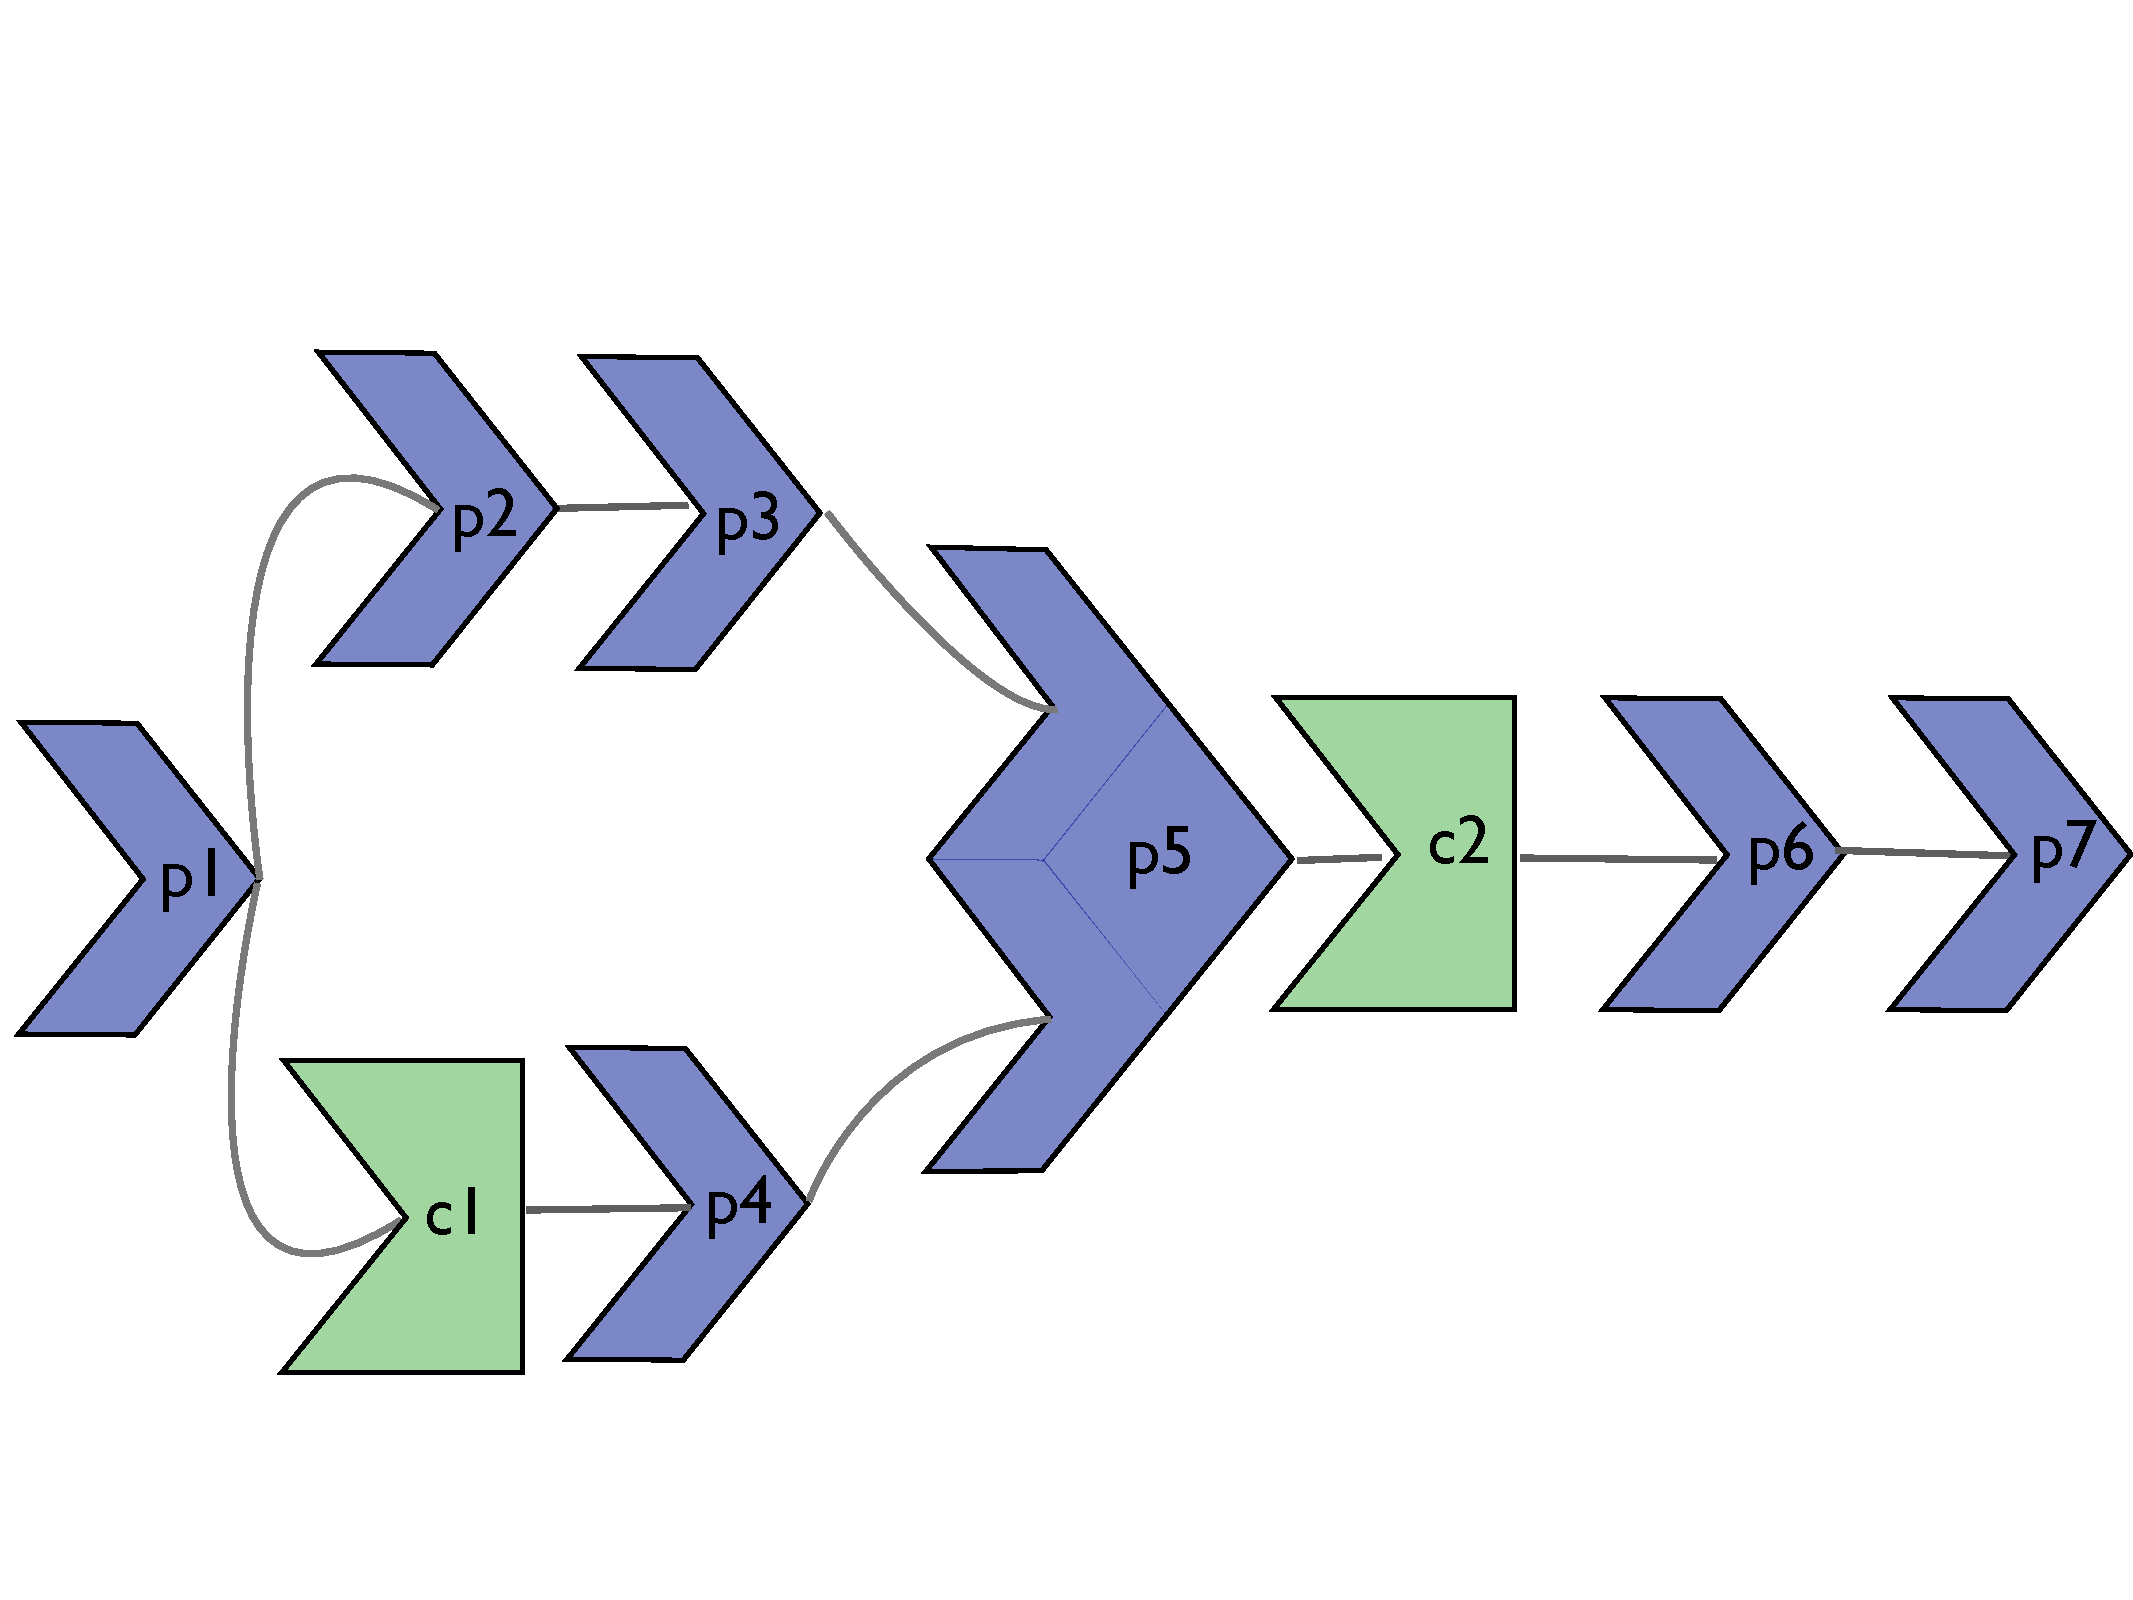
\includegraphics[scale=0.25]{images/sec-5/fusion1.pdf}
    \flushright \small(After producer/producer fusion)\qquad\\
    \centering  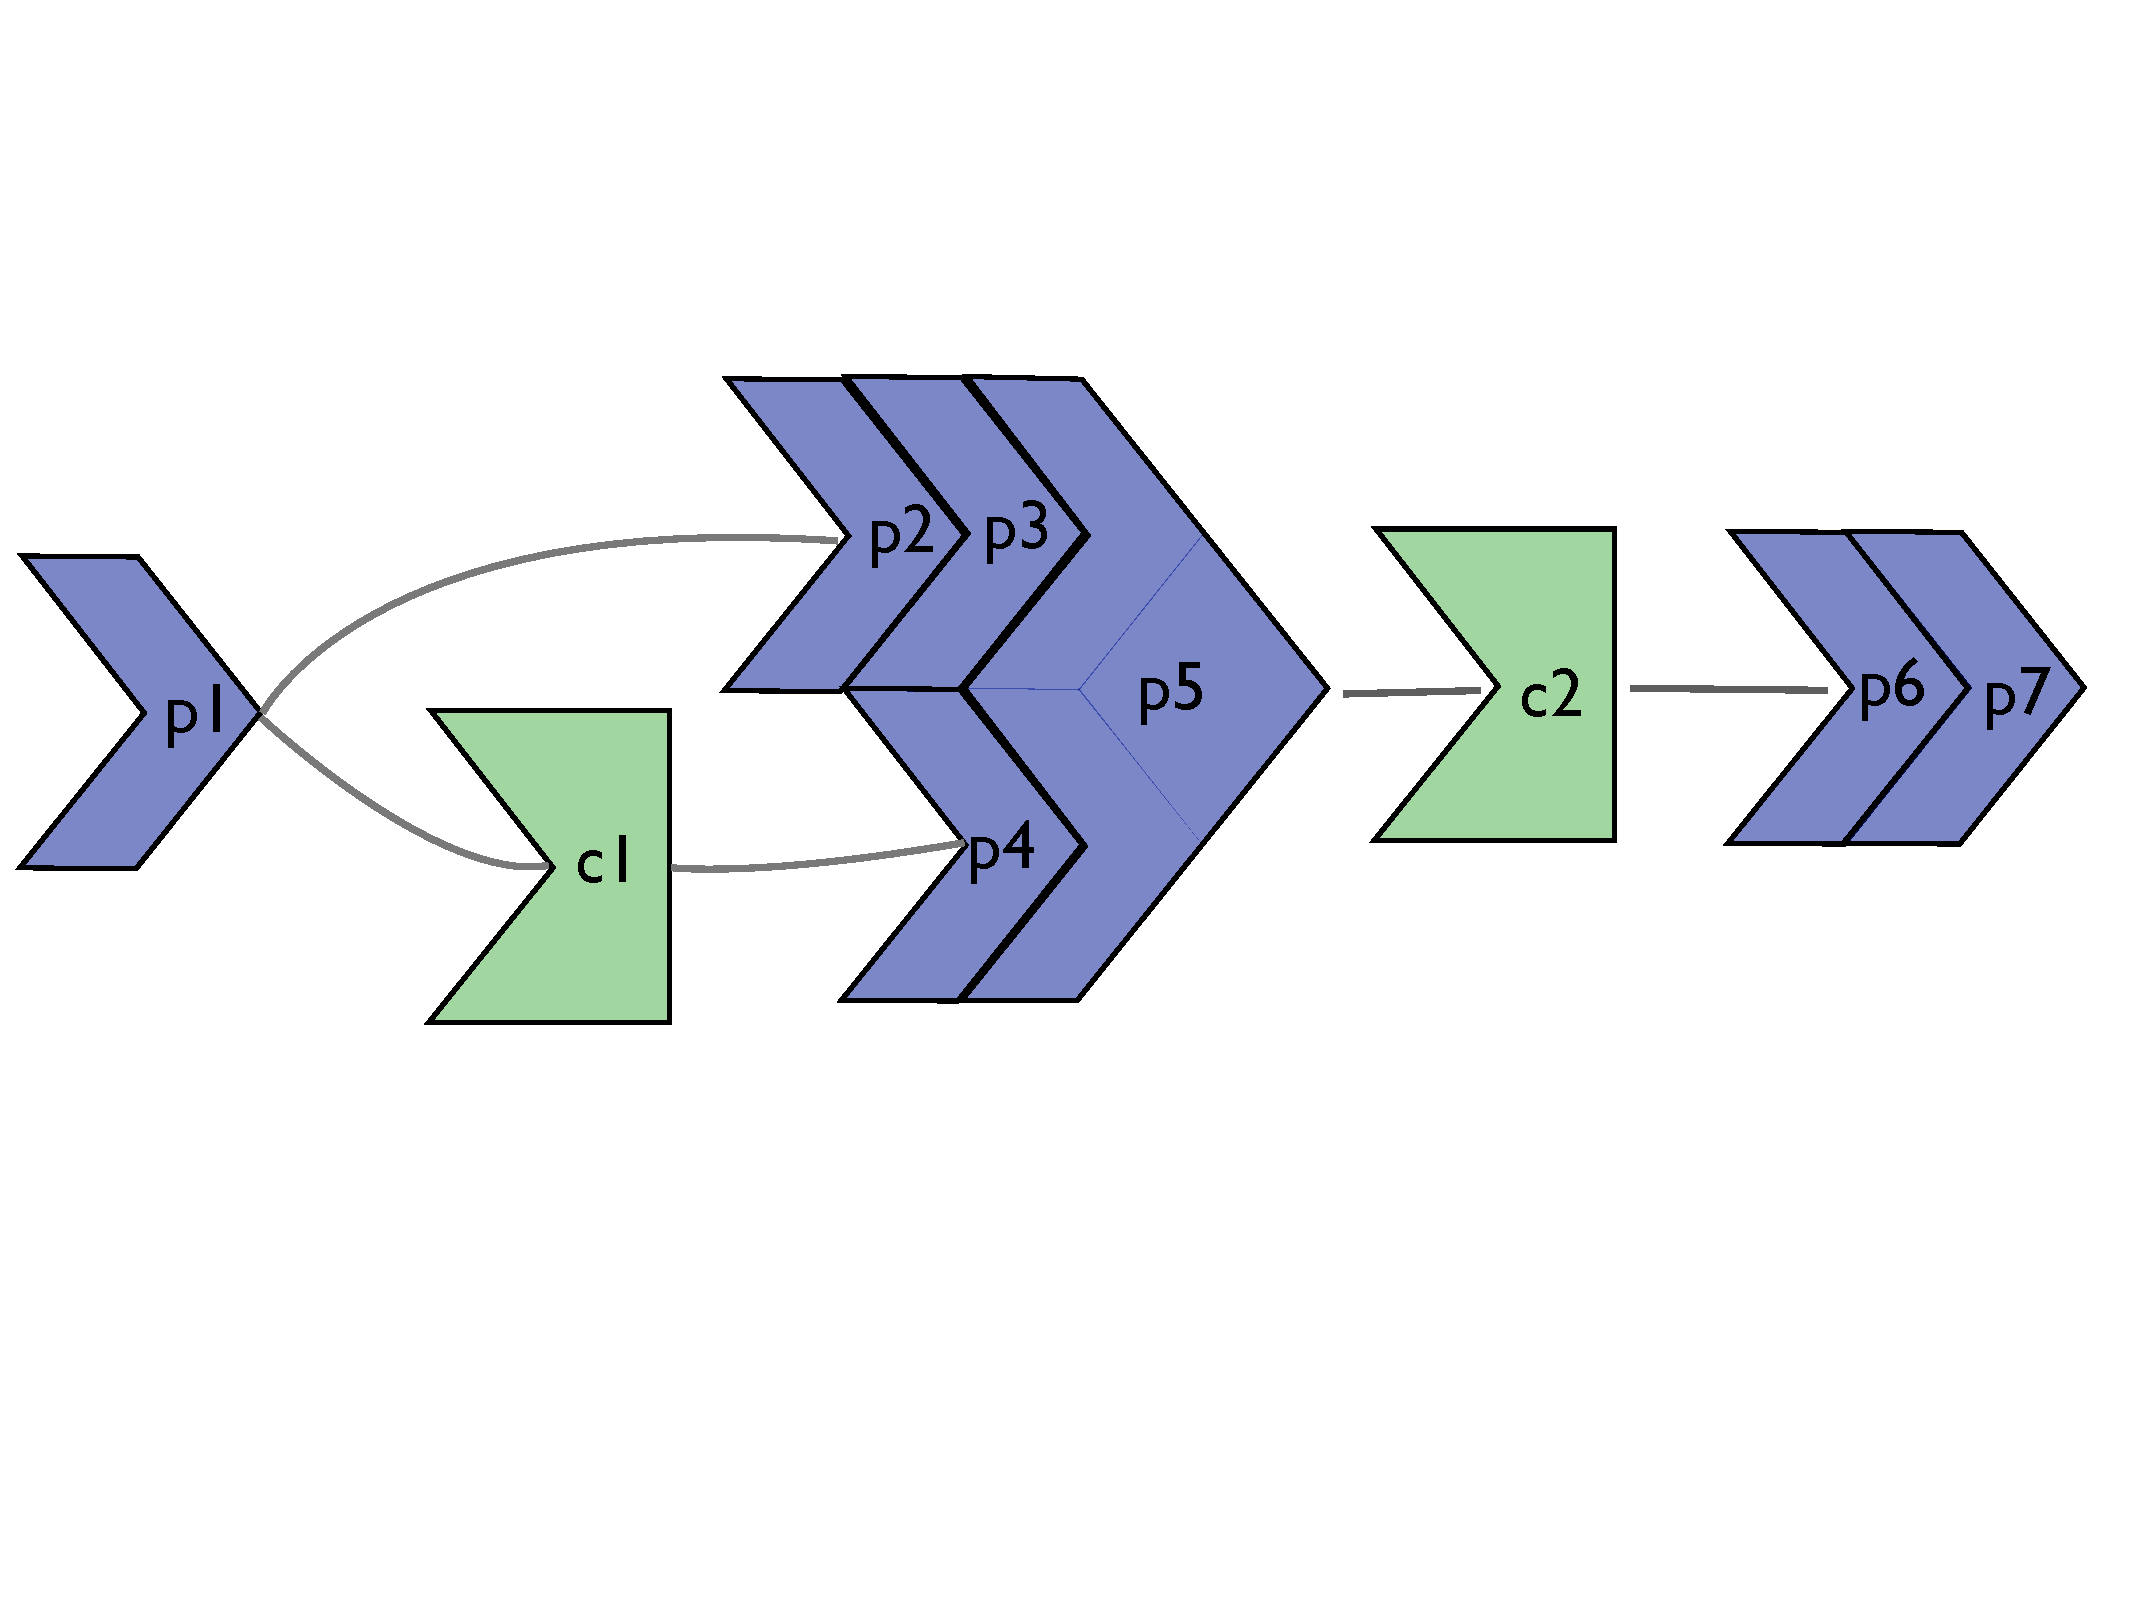
\includegraphics[scale=0.25]{images/sec-5/fusion2.pdf}
    \flushright \small(After producer/consumer fusion)\qquad\\
    \centering  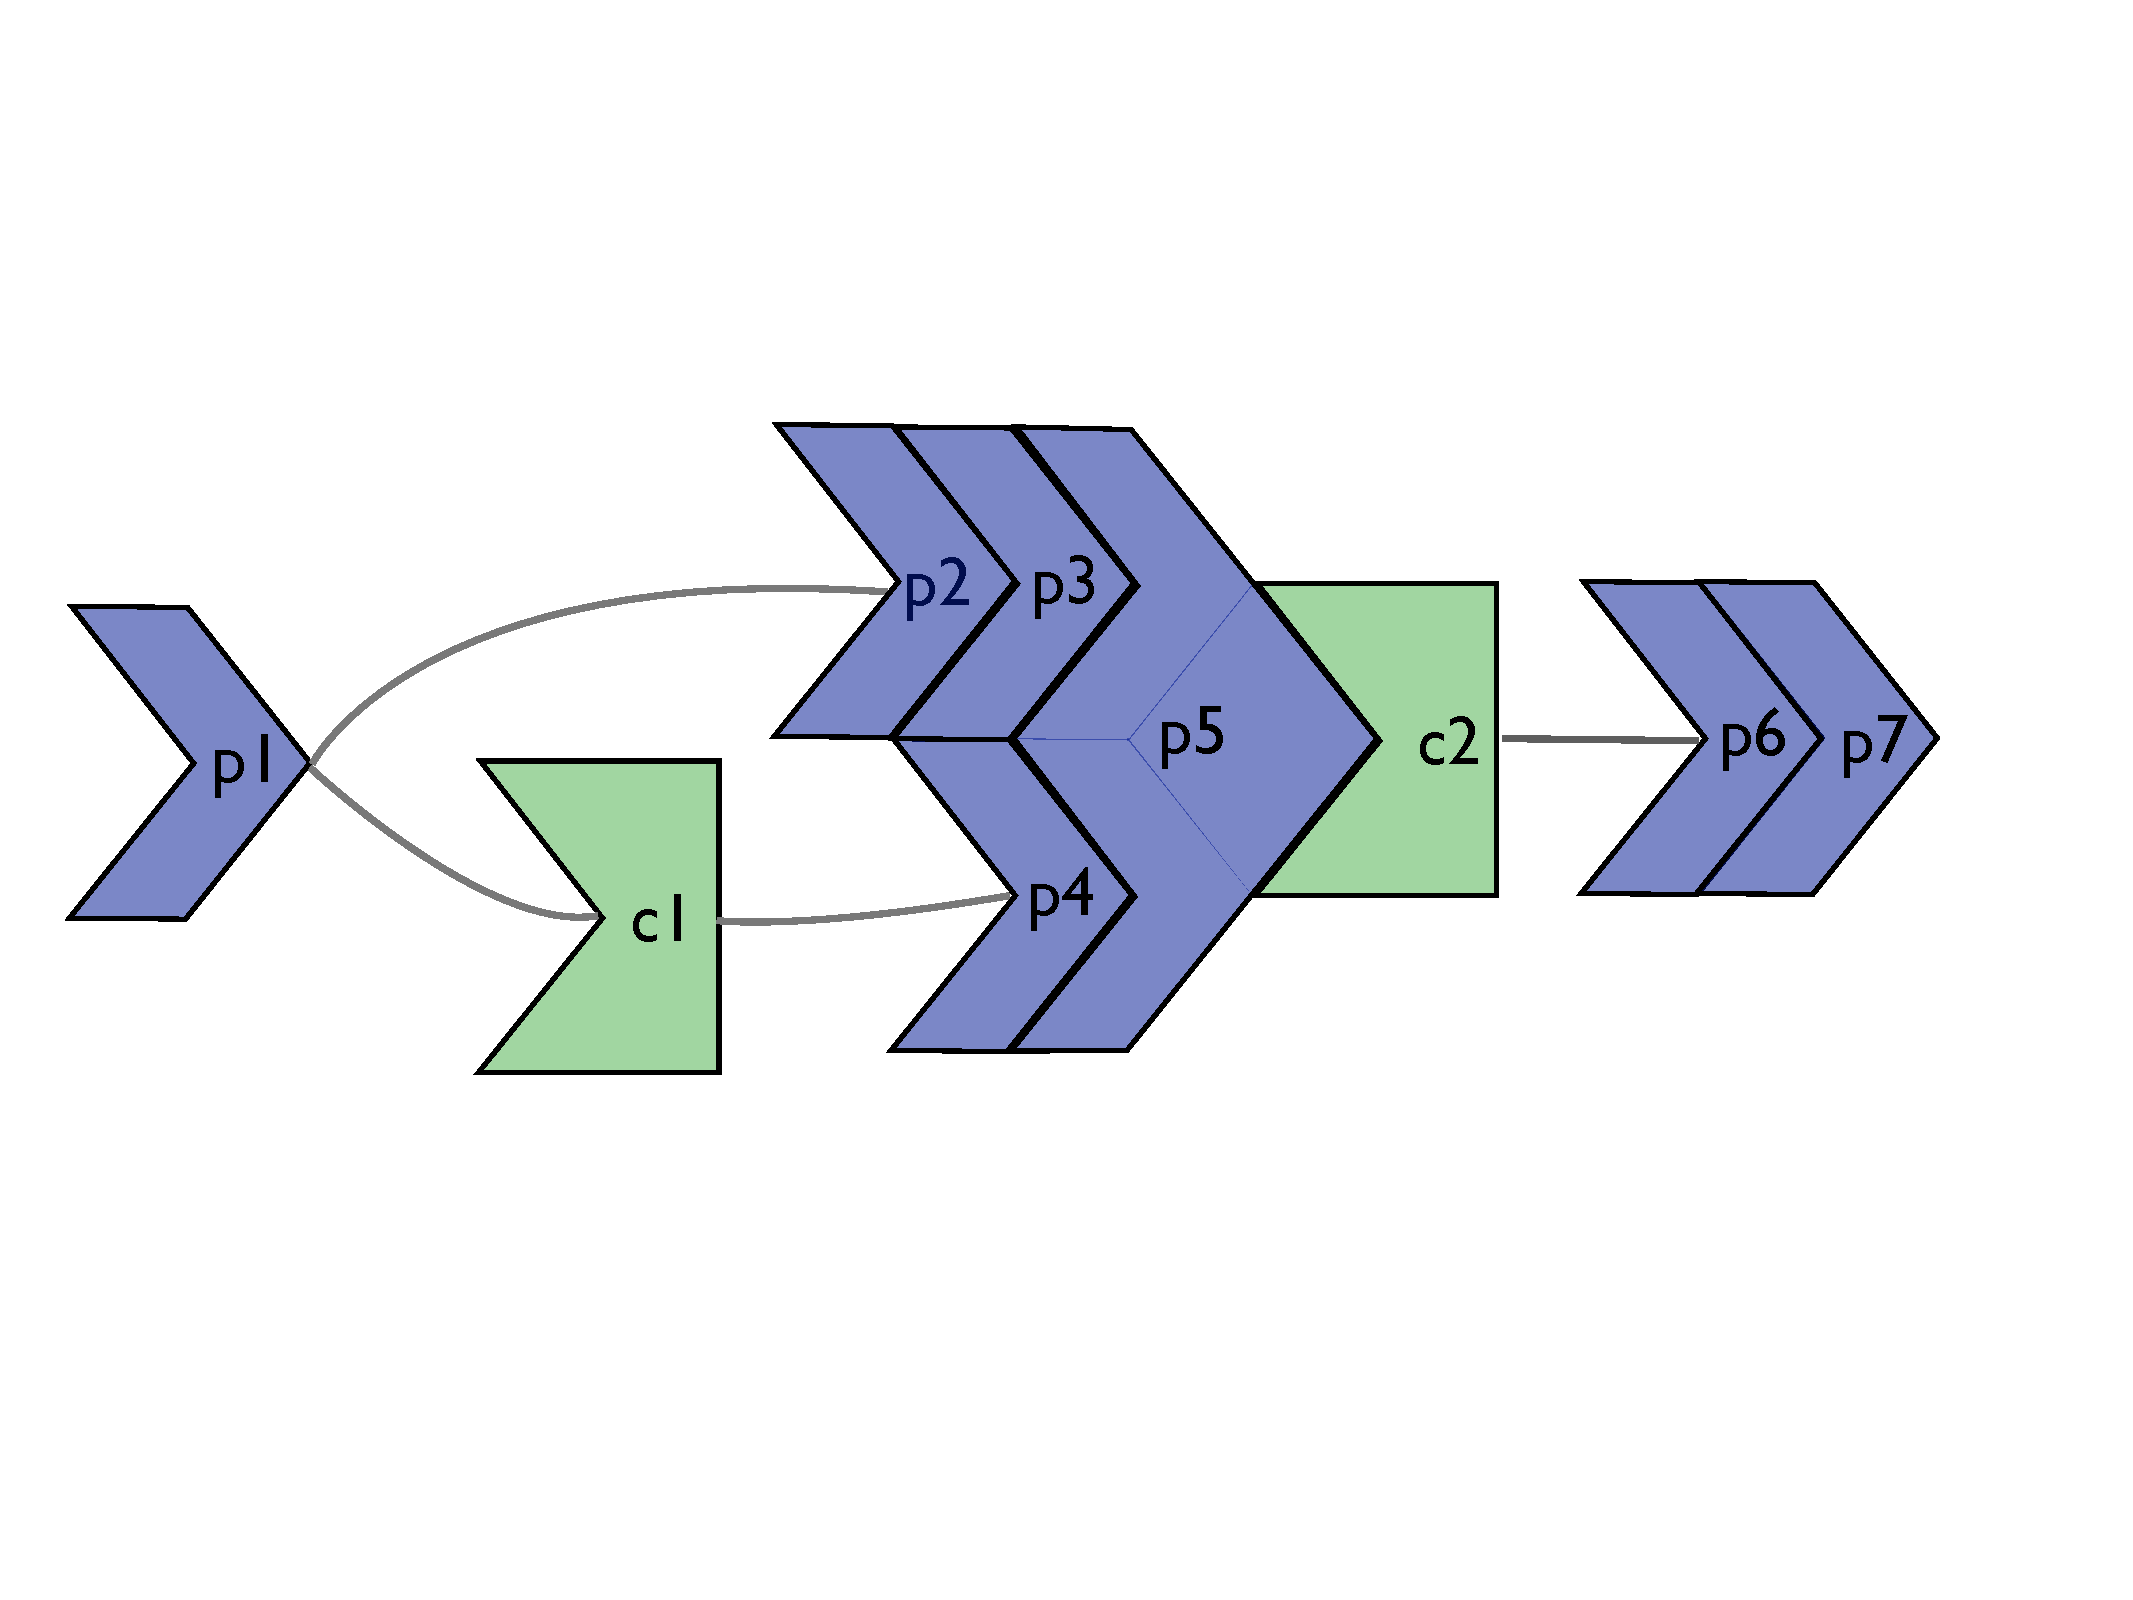
\includegraphics[scale=0.25]{images/sec-5/fusion3.pdf}
    \caption[Fusion in Accelerate]{Producer/producer and Producer/consumer fusion in Accelerate.}
    \label{fig:fusion}
\end{figure}

Figure~\ref{fig:fusion} shows how the fusion technique affects the
AST\index{abstract syntax tree}: blue boxes labelled $p_1$ to $p_7$ represent
producers, where $p_5$ is a producer like \code{zipWith} that takes two arrays
as input. The consumers are labelled $c_1$ and $c_2$. In the first phase all
adjacent producers are fused, with the exception of $p_1$ whose result is used
by both $c_1$ and $p_2$. In the second phase, the fused producers are embedded
into consumers where possible.

Throughout the transformation $p_1$ is left as is, as its result is used by both
$c_1$ and $p_2$. It would be straightforward to change the implementation such
that the work of $p_1$ is duplicated so that it can be used into both $p_2$ and
$c_1$. Despite reducing memory traffic, this is not always advantageous, so the
current implementation is conservative and never duplicates work. Since
Accelerate is a restricted, deeply embedded language, we can compute accurate
cost estimates and make an informed decision, but this is left for future work.
Moreover, this is an instance of a fundamental limitation with
\index{fusion!short-cut}short-cut fusion techniques such as
\index{fusion!foldr/build}\code{foldr/build} and \index{fusion!stream}stream
fusion. Since short-cut fusion is a local transformation that depends on
inlining, it is applicable only to fusing operations which have a single use
site. To implement this type of fusion efficiently would require fundamental
changes to the algorithm.
%
Producer/consumer fusion of $c_1$ into $p_4$, or $c_2$ into $p_6$, would also
require substantial changes to the fusion implementation.

Before discussing how to implement array fusion in Accelerate
(\S\ref{sec:implementing_array_fusion}), we take a brief detour to explain the
machinery that will be required in order to be able to manipulate terms and thus
implement the transformation.


\section{Typed Equality}
\label{sec:equality}
\marginnote{tk: into implementation chapter?}

The Accelerate core language is richly typed, maintaining full type information
of the embedded language in the term tree. In order to apply transformations to
these terms while maintaining the correctness of the program as encoded in its
type, we require methods to manipulate these richly typed terms in a type- and
scope-preserving manner.

For example, if we want to test whether two terms are equal to determine whether
the subexpressions can be shared, we immediately run into the problem that terms
are existentially typed:
%
\begin{lstlisting}[style=haskell]
Exp s == Exp t = ??
\end{lstlisting}
%
There is no reason that \code{s} and \code{t} should be expressions of the same
type. In some instances we might not care, and as such can define standard
heterogeneous equality:
%
\begin{lstlisting}[style=haskell]
instance Eq (PreOpenExp acc env aenv t) where
    (==) = heq
    where
        heq :: PreOpenExp acc env aenv a -> PreOpenExp acc env aenv b -> Bool
        heq = ...
\end{lstlisting}
%
where we do not care about the result type of each expression, and only require
that the environment type, re size, of free scalar and array variables are the
same so that we can test equality of \indext{de Bruijn} indices.

However, we often \emph{do} care about the specific types of our existentially
quantified terms. Consider the case of defining equality for let-bindings.
Recall:
%
\begin{lstlisting}[style=haskell]
data PreOpenExp acc env aenv t where

  -- Local binding of a scalar expression
  Let   :: (Elt bnd_t, Elt body_t)
        => PreOpenExp acc env          aenv bnd_t       -- bound term
        -> PreOpenExp acc (env, bnd_t) aenv body_t      -- body/scope of binding
        -> PreOpenExp acc env          aenv body_t
\end{lstlisting}
%
To apply \code{heq} to the body expression, we need to know something about
the type of the bound terms to ensure that the scalar environments are the same,
namely \lstinline[style=inline,mathescape]{a $\sim$ bnd_t $\sim$ b}.%
\footnote{Alternatively we can use \code{Data.Typeable.gcast} to provide a
type-safe cast, but this quickly becomes unwieldy and is a little
unsatisfactory.} To do this we must equip terms with a runtime witness to the
existentially quantified type. Our reified dictionaries will allow us to do
exactly this, so we can define heterogeneous equality for reified dictionaries:
%
\begin{lstlisting}[style=haskell]
heqIntegralType :: IntegralType s -> IntegralType t -> Bool
heqIntegralType (TypeInt _)  (TypeInt _)  = True
heqIntegralType (TypeWord _) (TypeWord _) = True
  ...
heqIntegralType _            _            = False
\end{lstlisting}
%
However, doing this is perfectly useless as it only gives us a value of type
\code{Bool}, with no idea what that value means or to what its truth might
entitle us. The type checker does not gain any useful knowledge about the types
the dictionaries \code{a} and \code{b} witness simply by knowing that
\code{heqIntegralType a b = True}. A boolean is a bit uninformative.

Instead, we can write essentially the same test, but in the positive case
deliver some \emph{evidence} that the types are equal:
%
\begin{lstlisting}[style=haskell]
data s :=: t where
  REFL :: s :=: s

matchIntegralType :: IntegralType s -> IntegralType t -> Maybe (s :=: t)
matchIntegralType (TypeInt _)  (TypeInt _)  = Just REFL
matchIntegralType (TypeWord _) (TypeWord _) = Just REFL
  ...
matchIntegralType _            _            = Nothing
\end{lstlisting}
%
Matching on \code{Just REFL} will inject the knowledge into the type
checker that the types \code{s} and \code{t} are the same. Now with our
evidence-producing heterogeneous equality test for reified dictionary families,
we can compare two terms and gain type-level knowledge when they witness the
same value-level types. These witnesses for existentially quantified types then
allow us to test for equality \emph{homogeneously}, ensuring that positive
results from singleton tests give the bonus of unifying types for other tests:
%
\begin{lstlisting}[style=haskell]
matchPreOpenExp :: PreOpenExp acc env aenv s -> PreOpenExp acc env aenv t -> Maybe (s :=: t)
matchPreOpenExp (Let x1 e1) (Let x2 e2)
  | Just REFL <- matchOpenExp x1 x2     -- if the bound expressions match
  , Just REFL <- matchOpenExp e1 e2     -- then the environment of the body term will also match
  = Just REFL

matchPreOpenExp ...
\end{lstlisting}


\subsection{Congruence}

As we are interested in the facility of matching terms for the purposes of
optimisations such as common subexpression elimination, it is beneficial to
define not equality but instead \indexe{congruence} of terms. Two nodes are
considered congruent if the nodes they label are constants and the constants are
equal; or they have the same operator and the operands are congruent. The crux
of the latter condition refers to commutative relations, such as scalar
addition, where an operator yields the same result when the order of the
operands are reversed. When checking equality of primitive applications, we
discriminate binary functions whose arguments commute, and return those
arguments in a stable ordering by comparing a hash of each of the
sub-terms.
%
\begin{lstlisting}[style=haskell]
commutes :: PrimFun (a -> r) -> PreOpenExp acc env aenv a -> Maybe (PreOpenExp acc env aenv a)
commutes f x = case f of
  PrimAdd _     -> Just (swizzle x)
    ...         -> Nothing
  where
    swizzle :: PreOpenExp acc env aenv (a,a) -> PreOpenExp acc env aenv (a,a)
    swizzle exp
      | Tuple (NilTup `SnocTup` a `SnocTup` b) <- exp
      , hashPreOpenExp a > hashPreOpenExp b     = Tuple (NilTup `SnocTup` b `SnocTup` a)
      | otherwise                               = exp
\end{lstlisting}


\section{Simultaneous Substitution}
\label{sec:substitution}
\marginnote{tk: into implementation chapter?}

In order to do things like renaming and substitution we require a value-level
substitution algorithm for the richly typed terms. The implementation follows
the method of \citet{McBride:2006up,McBride:2005jv}, where it is seen that
renaming and substitution are both instances of a \emph{single} traversal
operation, pushing functions from variables to ``stuff'' through terms, for a
suitable notion of stuff.
%
The trick is to push a \emph{type-preserving} but \emph{environment changing}
operation structurally through terms:
%
\begin{lstlisting}[style=haskell]
v :: forall t'. Idx env t' -> f env' t'
\end{lstlisting}

Where the operation differs is in the image of variables: renaming maps
variables to variables and substitution maps variables to terms. We then lift
this to an operation which traverses terms, with appropriate lifting to push
under a lambda, and rebuilding the term after applying \code{v} to the
variables:
%
\begin{lstlisting}[style=haskell]
rebuild :: Syntactic f
        => (forall t'. Idx env t' -> f env' t')
        -> Term env  t
        -> Term env' t
\end{lstlisting}

The \code{Syntactic} class\footnote{Since Accelerate is a stratified language
there are separate implementations of this toolkit on syntactic elements for the
scalar and collective operations, but the details are identical. The discussion
uses the generic \code{Term} to mean either of these operations.} tells us
everything we need to know about \code{f} --- our notion of ``stuff'' --- in
order to rebuild terms: a mapping in from variables, a mapping out to terms, and
a weakening map which extends the context. Renaming will instantiate \code{f}
with \code{Idx}, whereas for substitutions we may choose \code{Term} instead.
%
\begin{lstlisting}[style=haskell]
class Syntactic f where
    varIn   :: Idx env t -> f env t             -- variables embed in f
    termOut :: f env t   -> Term env t          -- f embeds in terms
    weaken  :: f env t   -> f (env, s) t        -- f allows weakening

instance Syntactic Idx
instance Syntactic Term
\end{lstlisting}

A key component of this toolkit, \indexe{weakening} describes an operation we
usually take for granted: every time we learn a new word, old sentences still
make sense; if a conclusion is justified by a hypothesis, it is still justified
if we add more hypotheses; a term remains in scope if we bind new (fresh)
variables. Weakening is the process of shifting things from one scope to a
larger scope in which new things have become meaningful, but no old things have
vanished. When we use a named representation (or HOAS\index{higher-order
abstract syntax}\index{HOAS|see{higher-order abstract syntax}}) we get weakening
for free, but in the de Bruijn\index{de Bruijn} representation weakening takes
work: we need to shift all the variable references to make room for new
bindings. To do this we need to explain how to shift the \code{v} operation into
an extended environment; saying what to do with the new variable and how to
account for it on the output side.
%
\begin{lstlisting}[style=haskell]
shift :: Syntactic f
      => (forall t'. Idx env t' -> f env' t')
      -> Idx (env,  s) t
      -> f   (env', s) t
\end{lstlisting}
%
Overall, the crucial functionality of simultaneous substitution is to propagate
a class of operations on variables closed under shifting, which is what
\code{Syntactic} and \code{rebuild} offer.


\subsection{Inlining}
\label{sec:inlining}

The final question, then, is how to write the function \code{v} which we push
through terms, as the type \code{forall t'} could be anything. After all, what
is the point of having a simultaneous substitution algorithm if we can't
specialise it to one-at-a-time substitution.

The following function takes a replacement for the top variable and returns a
simultaneous substitution which eliminates \code{ZeroIdx}.
%
\begin{lstlisting}[style=haskell
    ,name=inlining
    ,caption={[A simultaneous substitution to inline terms]}]
subTop :: Term env s -> Idx (env, s) t -> Term env t
subTop s ZeroIdx      = s
subTop _ (SuccIdx ix) = Var ix
\end{lstlisting}
%
If we have a term with one free variable, we can use this to replace that
variable with a term. That is, inline a term into all use sites of the free
variable.
%
\begin{lstlisting}[style=haskell,
    name=inlining,
    caption={A simultaneous substitution to inline terms}]
inline :: Term (env, s) t -> Term env s -> Term env t
inline body bnd = rebuild (subTop bnd) body
\end{lstlisting}
%
The demonic $\forall$ --- which is to say that the quantifier is in a position
which gives us obligation, not opportunity --- of the operator \code{v} forces
us to respect type: when pattern matching detects the variable we care about,
happily we discover that it has the type we must respect. The demon is not so
free to mess with us as one might at first fear.

% Typing rules; each rule types the general usage of a symbol, below the
% line, in terms of the parameters above the line.??

\subsection{Function composition}
\label{sec:function_composition}

The equivalent of unary function composition \code{(.)} on terms can be
defined in a similar manner. A function \code{(a -> b)} is equivalent to a
\code{Term} of type \code{b} and free variable \code{a}. Similar to inlining, we
replace an expression that uses the top variable with one that uses another,
remembering to bind the result of the first expression so that it can be reused
in the second without duplication.
%
\begin{lstlisting}[style=haskell
    ,name=function_composition
    ,caption={[A simultaneous substitution to compose unary function terms]}]
dot :: Term (env, b) c -> Term (env, a) b -> Term (env, a) c
dot f g = Let g (rebuild split f)
  where
    split :: Idx (env, b) c -> Term ((env, a), b) c
    split ZeroIdx      = Var ZeroIdx
    split (SuccIdx ix) = Var (SuccIdx (SuccIdx ix))
\end{lstlisting}
%
Note the type of \code{split}, where we needed to create space in the
environment at the second index (\code{SuccIdx ZeroIdx}) for the free variable
\code{a} to appear in the resultant \code{Term}, as the first index will be
bound to the result of the first expression \code{g}.

We lift this to function terms by unwrapping the lambda abstractions.
Annoyingly, GHC's type checker can not determine that the function type
prohibits any valid term except those with a single lambda, so we need a second
catch-all case to suppress a compilation warning. In future we elide the
impossible cases for brevity.
%
\begin{lstlisting}[style=haskell,
    name=function_composition,
    caption={A simultaneous substitution to compose unary function terms}]
compose :: Fun env (b -> c) -> Fun env (a -> b) -> Fun env (a -> c)
compose (Lam (Body f)) (Lam (Body g)) = Lam (Body (f `dot` g))
compose _              _              = error "compose: impossible case"
\end{lstlisting}


\section{Environment Manipulation}
\label{sec:environment_manipulation}
\marginnote{tk: into implementation chapter?}

As part of the fusion transformation of recasting terms we often need to lift
array valued inputs to be let-bound at higher points to avoid work duplication,
but at the same time we can not immediately add these bindings to the output
term because they will interfere with further fusion steps. We need to collect
these extra bindings separately from the main term, and add them to the output
term at some later point. Furthermore, we must ensure we correctly track the
types of the environments between the fused terms and the collected
let-bindings.

The following is a heterogeneous snoc-list of array terms that witnesses how an
array environment is extended by the application of these operations:
%
\begin{lstlisting}[
    style=haskell,
    label={lst:Extend},
    caption={Extending an array environment}]
data Extend acc aenv aenv' where
  BaseEnv :: Extend acc aenv aenv
  PushEnv :: Arrays a
          => Extend acc aenv aenv' -> PreOpenAcc acc aenv' a -> Extend acc aenv (aenv', a)
\end{lstlisting}
%
In the style of the \indext{de Bruijn} indices used for projecting environment
variables (\S TK), \code{Extend} uses an inductive notion of tuples as
heterogeneous \emph{snoc} lists. In contrast to environment indices, the base
case does not refer to an empty environment, but instead the environment
\code{aenv} which we are extending. This witnesses how to construct an extended
environment \code{aenv'} by bringing new terms into scope, one at a time.
%
\begin{lstlisting}[style=haskell]
bind :: Arrays a => Extend acc aenv aenv' -> PreOpenAcc acc aenv' a -> PreOpenAcc acc aenv a
bind BaseEnv         = id
bind (PushEnv env a) = bind env . Alet (inject a) . inject
\end{lstlisting}


\subsection{Sinking}
\label{sec:sinking}

We define \emph{sinking} as the operation of shifting a term from one (array)
environment into another, where new things have come into scope according to
some witness, and no old things have disappeared.
%
\begin{lstlisting}[style=haskell,
    name=sinking,
    caption={Sinking terms to a larger environment}]
type env :> env' = forall t'. Idx env t' -> Idx env' t'

class Sink f where
  weaken :: env :> env' -> f env t -> f env' t

instance Sink Idx
instance Sink (PreOpenExp acc env)
instance Sink (PreOpenAcc acc)
  ...
\end{lstlisting}
%
This generalises \code{weaken} from section~\ref{sec:substitution} to increase
the environment of an object \code{f} based on some function on indices rather
than shifting by a single \indext{de Bruijn} index. Thus we only need to
traverse a term once no matter how many positions the variable indices shift by.
Using this, we can weaken terms based on the witness provided by
\code{Extend}.
%
\begin{lstlisting}[style=haskell,name=sinking]
sink :: Sink f => Extend acc env env' -> f env t -> f env' t
sink env = weaken (k env)
  where
    k :: Extend acc env env' -> Idx env t -> Idx env' t
    k BaseEnv       = id
    k (PushEnv e _) = SuccIdx . k e

sink1 :: Sink f => Extend acc env env' -> f (env, s) t -> f (env', s) t
sink1 = ...
\end{lstlisting}


\section{Implementing Array Fusion}
\label{sec:implementing_array_fusion}
\marginnote{tk: describe Kit? else drop references to it}

Section~\ref{sec:fusion} outlined the basic approach to fusion. To reiterate, we
partition array operations into two categories as per
Listing~\ref{lst:operations}:
%
\begin{enumerate}
    \item \index{producer}\emph{Producer} operations consist of independent
        element-wise operations which have an obvious parallel implementation.
%        Successive producer operations are fused together.

    \item \index{consumer}\emph{Consumer} operations manipulate multiple
        elements of the input or output array and so are less straightforward.
        Efficient parallel implementation needs to know exactly how elements
        depend on each other.
\end{enumerate}
%
As we saw in Figure~\ref{fig:fusion}, whenever possible successive producer
operations are fused together ($p_2$, $p_3$, $p_4$ and $p_5$), and producers are
fused into consumers ($p_{ 2,3,4,5 }$ into $ c_2$). We do not fuse the results
of consumers into subsequent producers ($c_2$ is not fused into $p_{ 6,7 }$).
% This has the happy consequence of maintaining trickiest parts of the parallel
% interpretation of the program.

We require a representation that will facilitate embedding of (fused) producer
terms into consumers. We do not wish to manipulate source terms directly, as
this would require a number of rewrite rules quadratic in the number of
operations that are to be fused. This was the problem with Wadler's original
deforestation algorithm. The representation must also be sufficiently expressive
to represent all operations we want to fuse, which was a limitation of
\index{fusion!foldr/build}\code{foldr/build} fusion.


\subsection{Representing Producers}
\label{sec:representing_producers}

The basic idea behind the representation of producer arrays in Accelerate is
well known: simply represent an array by its shape and a function mapping array
indices to their corresponding values. This method is used successively to
optimise purely functional array programs in \index{fusion!delayed
arrays}Repa~\cite{Keller:2010er}, and has also been used by
others~\cite{Claessen:2012hl}.

The use of delayed arrays [in Repa] was originally motived by the desire to
avoid superfluous copying of array elements during index space transformations
such as \code{backpermute} (see Listing~\ref{lst:operations}). Another major
benefit of delayed arrays is that it offers by-default automatic fusion.
Moreover, this fusion does not require sophisticated compiler transformations or
for the two fusible terms to be statically juxtaposed; fusion is a property of
the data representation.

Automatic fusion sounds too good to be true, and indeed it is. There are at
least two reasons why it is not always beneficial to represent all array terms
uniformly as functions. The first issue is \emph{sharing}. Consider the
following:
%
\begin{lstlisting}[style=haskell]
let b = map f a
in  mmMult b b
\end{lstlisting}
%
Every access to an element \code{b} will apply the (arbitrarily expensive)
function \code{f} to the corresponding element of \code{a}. It follows that
these arbitrarily expensive computations will be done \emph{at least twice},
once for each argument of \code{mmMult}, quite contrary to the programmer's
intent. Indeed, if \code{mmMult} consumes its elements in a non-linear manner,
accessing elements more than once, the computation of \code{f} will be performed
every time. We must be able to represent some terms as manifest arrays so that a
delayed-by-default representation can not lead to an arbitrary loss of sharing.
This is a well known problem with Repa.

The other consideration is \emph{efficiency}. Since we are targeting a massively
parallel architecture designed for performance, it is better to use more
specific operations whenever possible. An opaque indexing function is too
general, conveying no information about the pattern in which the underlying
array is accessed, and hence no opportunities for optimisation.

The following describes the ways in which the fusion transformation represents
intermediate arrays. The fusion process operates by recasting producer array
computations in terms of a set of scalar functions used to construct an element
at each index, % encoded by this data structure,
and fusing successive producers by combining these scalar functions. It is
defined as:
%
\begin{lstlisting}[style=haskell
    ,label=lst:cunctation
    ,caption={Representation of fusible producer arrays}]
data Cunctation acc aenv a where
  Done  :: Arrays a
        => Idx            aenv a                -- manifest array(s)
        -> Cunctation acc aenv a

  Yield :: (Shape sh, Elt e)
        => PreExp     acc aenv sh               -- output shape
        -> PreFun     acc aenv (sh -> e)        -- compute an element at each index
        -> Cunctation acc aenv (Array sh e)

  Step  :: (Shape sh, Shape sh', Elt a, Elt b)
        => PreExp     acc aenv sh'              -- output shape
        -> PreFun     acc aenv (sh' -> sh)      -- backwards permutation into input array
        -> PreFun     acc aenv (a   -> b)       -- function to apply to input value
        -> Idx            aenv (Array sh  a)    -- manifest input array
        -> Cunctation acc aenv (Array sh' b)
\end{lstlisting}
%
The representation\footnote{
cunc$\cdot$ta$\cdot$tion
\textcolor{gray}{|
k\textipa{@}NGk\textquotesingle t\={a}SH\textipa{@}n
\enspace\textipa{k@Nk}\textquotesingle \textipa{te\;IS@n}
|} (n) the action or an instance of delaying; tardy action.}
%
is parameterised by the recursive closure of array computations \code{acc}, the
array environment \code{aenv}, and has three constructors:
%
\begin{itemize}
\item \code{Done} injects a manifest array into the type.
    %represented as a reference to a term in the array environment.

\item \code{Yield} defines a new array in terms of its shape and a function
    that maps indices to elements.

\item \code{Step} encodes a special case of \code{Yield}, that defines a new
    array by applying an index and value transformation to an argument array.

\end{itemize}

Note that the argument arrays to \code{Done} and \code{Step} are not expressed
as terms in \code{acc}, the type of collective array operations. By instead
requiring a \indext{de Bruijn} index \code{Idx} into the array environment, we
ensure that the argument array is manifest. Thus the definition of
\code{Cunctation} is non-recursive in the type of array computations. This
allows the representation to be (later) embedded within producer terms
(\ref{sec:producer_consumer_fusion}) with the guarantee that an embedded scalar
computation will not invoke further parallel computations.%
\footnote{While scalar expression terms are mutually recursive in \code{acc},
we are guaranteed that these terms will consist only of free array variables
(\code{Idx}).}

In order to bring additional array terms into scope, which may be required for
\code{Done} and \code{Step}, we combine this representation of producer
arrays with the method of section~\ref{sec:environment_manipulation} for
collecting supplementary environment bindings. This completes our data structure
for combining producer terms in Accelerate:
%
\begin{lstlisting}[style=haskell
    ,label=lst:Embed
    ,caption={Representation of fused producer arrays in Accelerate}]
data Embed acc aenv a where
  Embed :: Extend     acc aenv aenv'            -- additional bindings to bring into scope, to evaluate the\ldots
        -> Cunctation acc      aenv' a          -- \ldots representation of (fused) producer terms
        -> Embed      acc aenv       a
\end{lstlisting}

Note the types of the array environments. The \code{Embed} type is expressed in
relation to the type \code{aenv}, which represents all let-bindings
currently in scope at this point of the AST\index{abstract syntax tree} that we
are currently fusing. The data constructor contains an existentially typed
\code{aenv'}, witnessed by the first argument, \code{Extend}, which contains any
supplementary array terms collected during the fusion process. The actual array
representation in the second argument is expressed in terms of this extended
environment, so has access to any terms from the AST (\code{aenv}) as well as
those additional bindings introduced by \code{Extend}.

Why do we separate the auxiliary bindings from the representation of fused
producers? The constructors of \code{Cunctation} could carry this information,
and then we would not require this additional data structure. For example, the
following is a valid alternative definition for the \code{Yield} constructor:
%
\begin{lstlisting}[style=haskell]
  Yield' :: (Shape sh, Elt e)                           -- Alternative definition (bad)
         => Extend     acc aenv aenv'                   -- NEW: supplementary environment bindings
         -> PreExp     acc      aenv' sh                -- CHANGED: terms now defined w.r.t. \texttt{aenv'}
         -> PreFun     acc      aenv' (sh -> e)
         -> Cunctation acc aenv       (Array sh e)
\end{lstlisting}

To create a real AST\index{abstract syntax tree} node from the \code{Embed}
representation, we need both the environment bindings as well as the array
description. However, analysis of how to fuse terms requires only the array
description. If the additional bindings are bundled as part of the array
representation, as in \code{Yield'}, the existentially quantified environment
type is only available after we pattern match on the constructor. This is
problematic because to inspect terms and do things like function composition
(\S\ref{sec:function_composition}) the types of the environments of the two
terms must be the same, so after we pattern match on the constructor we must
\code{sink} (\S\ref{sec:sinking}) the second term into \code{aenv'}. Even worse,
for terms in the delayed state the only way to do this sinking is to first
convert them into a real AST node and then back into the delayed state. If for
some reason we can not fuse into this representation --- for example we do not
meet the requirements for the more restrictive \code{Step} --- then this
additional work is wasted.

Why can we not analyse terms with respect to the exposed environment type
\code{aenv}, ignoring for the moment the existential? At some point we will need
to combine the extended environments, and we have no way to do this even if the
existential types are exposed.
%
\begin{lstlisting}[style=haskell]
cat :: Extend env env1 -> Extend env env2 -> Extend env ???
\end{lstlisting}

Because of the limited scope in which this existential type is available, we
ultimately perform this process of converting terms and sinking into a suitable
type many times. If the extended environments are placed on the constructors of
the delayed representations, the complexity of the fusion algorithm for an AST
of $n$ nodes scales as $O(r^n)$, where $r$ is the number of different rules we
have for combining delayed terms. While the semantics of the algorithm
ultimately remain the same, for performance reasons this separation is critical.

Finally, we convert the delayed representations into manifest data using the
\code{compute} function. It inspects the argument terms of the representation to
identify special cases, such as \code{map}s or \code{backpermute}s.
%
\begin{lstlisting}[style=haskell
    ,label=lst:compute
    ,caption={Computing the delayed representation to a manifest array}]
compute :: Arrays arrs => Embed acc aenv arrs -> PreOpenAcc acc aenv arrs
compute (Embed env cc) = bind env (compute' cc)

compute' :: Arrays arrs => Cunctation acc aenv arrs -> PreOpenAcc acc aenv arrs
compute' cc = case simplify cc of
  Done v                                   -> Avar v
  Yield sh f                               -> Generate sh f
  Step sh p f v
    | Just REFL <- match sh (arrayShape v)
    , Just REFL <- isIdentity p
    , Just REFL <- isIdentity f            -> Avar v                       -- unmodified manifest array
    | Just REFL <- match sh (arrayShape v)
    , Just REFL <- isIdentity p            -> Map f (avarIn v)             -- linear indexing OK
    | Just REFL <- isIdentity f            -> Backpermute sh p (avarIn v)  -- pure index transform
    | otherwise                            -> Transform sh p f (avarIn v)  -- index \& value transform
\end{lstlisting}

The helper functions \code{match} and \code{isIdentity} check for congruence of
expressions. As discussed in section~\ref{sec:equality}, we match on \code{Just
REFL} to inject information on the positive case to both the type and value
level. For example, \code{isIdentity} checks whether a function corresponds to
the term $\lambda x.x$, and in the positive case witnesses that its type must be
\code{a -> a}.


\subsection{Producer/Producer Fusion}
\label{sec:producer_producer_fusion}
% TK: rules for each of the smart constructors? kinda obvious once the
% representation is established

Producer/producer fusion is achieved by converting terms into the array
representation discussed in the previous section
(\S\ref{sec:representing_producers}), and merging sequences of producers into a
single operations. Smart constructors for each producer term manage the
integration with successive producers. For example, the following is the fused
version of \code{map}:
%
\begin{lstlisting}[style=haskell,
    caption={Fused definition of the \code{map} operation},
    label=lst:mapD]
mapD :: Elt b
     => PreFun     acc aenv (a -> b)
     -> Cunctation acc aenv (Array sh a)
     -> Cunctation acc aenv (Array sh b)
mapD f (step  -> Just (Step sh ix g v)) = Step sh ix (f `compose` g) v
mapD f (yield -> Yield sh g)            = Yield sh (f `compose` g)
\end{lstlisting}

We use two helper functions, \code{step} and \code{yield}, to expose the only
two interesting cases and then compose (\S\ref{sec:function_composition}) the
input function \code{f} into the appropriate place in the constructor. Index
transformation functions such as \code{backpermute} proceed in the same manner.

These helper functions operate by converting the input \code{Cunctation} into
the constructor with the same name. A producer can always be expressed as a
function from indices to elements in the style of \code{Yield}, but this is not
the case for the more restrictive \code{Step}. For the \code{Done} case in both
instances, GHC can not infer that the result type is a single \code{Array}, so
we use the \code{accType} function to reify the \code{Arrays} class
representation.
%
\begin{lstlisting}[style=haskell]
yield :: Cunctation acc aenv (Array sh e) -> Cunctation acc aenv (Array sh e)
yield cc = case cc of
  Yield{}                              -> cc
  Step sh p f v                        -> Yield sh (f `compose` indexArray v `compose` p)
  Done v | ArraysRarray <- accType' cc -> Yield (arrayShape v) (indexArray v)

step :: Cunctation acc aenv (Array sh e) -> Maybe (Cunctation acc aenv (Array sh e))
step cc = case cc of
  Yield{}                              -> Nothing
  Step{}                               -> Just cc
  Done v | ArraysRarray <- accType' cc -> Just $ Step (arrayShape v) identity identity v
\end{lstlisting}

The only interesting case is that of \code{zipWith}, which is the only producer
that consumes multiple arrays (see Listing~\ref{lst:operations}). In contrast
to, for example, \code{foldr/build}\index{fusion!foldr/build}, we fuse in both
of the input arguments.
%
\begin{lstlisting}[style=haskell
    ,name=zipWithD
    ,caption={[Fused definition of the \code{zipWith} operation]}]
zipWithD :: (Shape sh, Elt a, Elt b, Elt c)
         => PreFun     acc aenv (a -> b -> c)
         -> Cunctation acc aenv (Array sh a)
         -> Cunctation acc aenv (Array sh b)
         -> Cunctation acc aenv (Array sh c)
zipWithD f cc1 cc0
\end{lstlisting}
%
Because it is advantageous to express operations in the most specific way
possible, \code{zipWith} considers the special case of when the two input arrays
happen to derive from the same manifest data:
%
\begin{lstlisting}[style=haskell,name=zipWithD]
  | Just (Step sh1 p1 f1 v1)    <- step cc1
  , Just (Step sh0 p0 f0 v0)    <- step cc0
  , Just REFL                   <- match v1 v0
  , Just REFL                   <- match p1 p0
  = Step (sh1 `Intersect` sh0) p0 (combine f f1 f0) v0
\end{lstlisting}
%
In general, we simply convert both inputs into functions from indices to
elements and combine:
%
\begin{lstlisting}[style=haskell,name=zipWithD]
  | Yield sh1 f1                <- yield cc1
  , Yield sh0 f0                <- yield cc0
  = Yield (sh1 `Intersect` sh0) (combine f f1 f0)
\end{lstlisting}
%
The function \code{combine} completes the task of drawing an element from each
of the input arrays and combining them with the binary function \code{f}, being
sure to let-bind the intermediate results along the way.
%
\begin{lstlisting}[style=haskell
    ,name=zipWithD
    ,caption={Fused definition of the \code{zipWith} operation}
    ,escapeinside={(*}{*)}]
  where
    combine :: forall acc aenv a b c e. (Elt a, Elt b, Elt c)
            => PreFun acc aenv (a -> b -> c)
            -> PreFun acc aenv (e -> a)
            -> PreFun acc aenv (e -> b)
            -> PreFun acc aenv (e -> c)
    combine c ixa ixb
      | Lam (Lam (Body c'))     <- weakenFE SuccIdx c   :: PreOpenFun acc ((),e) aenv (a -> b -> c) (*\label{lst:zipwithD_combine_weaken}*)
      , Lam (Body ixa')         <- ixa
      , Lam (Body ixb')         <- ixb
      = Lam $ Body $ Let ixa' $ Let (weakenE SuccIdx ixb') c'
\end{lstlisting}
%
Note that line~\ref{lst:zipwithD_combine_weaken} requires a type signature,
otherwise the type variable \code{e} introduced by the weakening step will
escape and can not be unified correctly. This new parameter \code{e} represents
in the first case of \code{Step} the array element type, and in the second
instance via \code{Yield} the array index type.


\subsubsection{Step 1: Fusing Producers}
\label{sec:fusing_producers}

The first phase of fusion completes via bottom-up tree contraction of the
AST\index{abstract syntax tree}. Terms are converted into the intermediate
representation and merged as described in the previous section
(\S\ref{sec:producer_consumer_fusion}). The following example demonstrates the
procedure for a producer (\code{map}), a consumer (\code{fold}) as well as a
non-computation form (\code{use}). Non-computation forms may also employ smart
constructors, the most interesting of which is that for let-bindings, although
we defer that discussion until section~\ref{sec:binder_elimination}.
%
\begin{lstlisting}[style=haskell
    ,name=embedPreAcc
    ,label=lst:embedPreAcc
    ,caption={[Producer fusion via bottom-up contraction of the AST]}]
embedPreAcc :: PreOpenAcc acc aenv arrs -> Embed acc aenv arrs
embedPreAcc pacc =
  case pacc of
    Alet bnd body       -> aletD bnd body                               -- see section~\ref{sec:binder_elimination}
    Use arrs            -> done  (Use arrs)                             -- non-computation node
    Map f a             -> fuse  (into  mapD (cvtF f)) a                -- producers
    Fold f z a          -> embed (into2 Fold (cvtF f) (cvtE z)) a       -- consumers
    ...
\end{lstlisting}

The function \code{done} simply converts an AST node into the internal
representation as a manifest array. This also illustrates why we require both
\code{Done} and \code{Step} representations. It would be convenient to represent
manifest data as \code{Step} with identity transformation functions, but the
result type of \code{Step} is restricted to a single \code{Array}, whereas
\code{Done} generalises to any instance of the \code{Arrays} class.

\begin{lstlisting}[style=haskell,name=embedPreAcc]
  where
    done :: Arrays a => PreOpenAcc acc aenv a -> Embed acc aenv a
    done (Avar v) = Embed BaseEnv                  (Done v)
    done pacc     = Embed (BaseEnv `PushEnv` pacc) (Done ZeroIdx)
\end{lstlisting}

In order to use our smart constructors for producer terms, such as \code{mapD}
(Listing~\ref{lst:mapD}), all of the terms must be expressed with respect to the
same array environment. This simplifies the definition of the fusion rules, but
recall that the representation of producer arrays includes additional array
environment bindings (see section~\ref{sec:representing_producers}). The
function \code{into} is used to convert a function of one type-annotated
argument into a function of one argument \emph{plus} a witness that sinks the
argument from one environment type into another.

\begin{lstlisting}[style=haskell,name=embedPreAcc]
    into :: Sink f => (f env' a -> b) -> f env a -> Extend acc env env' -> b
    into op a env = op (sink env a)
\end{lstlisting}

In the example, \code{into} is partially applied with the smart constructor
\code{mapD} and the scalar function applied at each element. This result is
passed to \code{fuse} which does the work of traversing the AST\index{abstract
syntax tree} bottom-up to produce the fused \code{Embed} representation. The
modified \code{mapD} is saturated with the extra environment bindings and the
array representation, to produce a new delayed representation that can be
further fused into later terms.

\begin{lstlisting}[style=haskell,name=embedPreAcc]
    fuse :: Arrays as
         => (forall aenv'. Extend acc aenv aenv' -> Cunctation acc aenv' as -> Cunctation acc aenv' bs)
         ->       acc aenv as
         -> Embed acc aenv bs
    fuse op (embedAcc -> Embed env cc) = Embed env (op env cc)
\end{lstlisting}

In contrast to \code{fuse}, which allows the result to be combined with later
terms, the \code{embed} function instead evaluates the argument array at this
point in the program to a manifest array. This is achieved by converting the
\code{Embed} representation into a real AST\index{abstract syntax tree} node
using \code{compute'} (see Listing~\ref{lst:compute}). The only point of note is
that the argument array (\code{cc}) is placed adjacent to the term consuming it
(\code{op}), which is important for the second fusion phase discussed in the
next section (\S\ref{sec:producer_consumer_fusion}).

\begin{lstlisting}[style=haskell
    ,name=embedPreAcc
    ,caption={Producer fusion via bottom-up contraction of the AST}]
    embed :: (Arrays as, Arrays bs)
          => (forall aenv'. Extend acc aenv aenv' -> acc aenv' as -> PreOpenAcc acc aenv' bs)
          ->       acc aenv as
          -> Embed acc aenv bs
    embed op (embedAcc -> Embed env cc) =
      = Embed (env `PushEnv` op env (inject (compute' cc))) (Done ZeroIdx)
\end{lstlisting}

\subsection{Producer/Consumer Fusion}
\label{sec:producer_consumer_fusion}
% TK: The Delayed type and embedding producers into consumers (second phase of
% fusion)

Now that we have a story for producer/producer fusion, we discuss how to deal
with consumers. The classic array fusion example is that of vector dot product:

\begin{lstlisting}[style=haskell,label=lst:dotp]
dotp :: Acc (Vector Float) -> Acc (Vector Float) -> Acc (Scalar Float)
dotp xs ys = A.fold (+) 0                       -- sum result of\ldots
           $ A.zipWith (*) xs ys                -- \ldots element-wise multiplying inputs
\end{lstlisting}
%
This consists of two collective operations: the first multiplies values from the
two input arrays element-wise, and the second sums this result. The fusion
system should translate this into a single collective operation, in much the
same way as a human would write if working directly in a low-level language such
as C or CUDA.

The basic idea is to pass producers encoded in the \code{Cunctation}
representation directly to consumers, and implementation of the consumer can
decide how best to access values of the input. Consumers themselves have no
\code{Cunctation} representation, however.

Consumers such as \code{stencil} apply a function with access to all array
elements within a local neighbourhood of the focal point of the stencil. As
overlapping stencils from neighbouring elements access the same elements in
their argument arrays many times, they must be implemented carefully not to
duplicate work. Even when the argument of such a consumer is a manifest array,
the consumer should still ensure that it caches already fetched elements, as
GPUs impose a high performance penalty for repeated memory access. So, stencil
operations fully compute their input array(s) before evaluating their outputs.
On the other hand, some consumers can be implemented more efficiently when given
a producer that is expressed in terms of a function from a multi-dimensional
array index to an element value, so that the elements the consumer needs are
generated on-the-fly instead of simply read from manifest data. Other consumers
can be further optimised by utilising functions that map the flat linear index
of the underlying array to its value. The consumer friendly representation
therefore contains all of these versions:

\begin{lstlisting}[style=haskell
    ,name=DelayedOpenAcc
    ,label=lst:DelayedOpenAcc
    ,caption={The type of delayed arrays in Accelerate}]
data DelayedOpenAcc aenv a where
  Manifest              :: PreOpenAcc DelayedOpenAcc aenv a -> DelayedOpenAcc aenv a

  Delayed               :: (Shape sh, Elt e) =>
    { extentD           :: PreExp DelayedOpenAcc aenv sh
    , indexD            :: PreFun DelayedOpenAcc aenv (sh  -> e)
    , linearIndexD      :: PreFun DelayedOpenAcc aenv (Int -> e)
    }                   -> DelayedOpenAcc aenv (Array sh e)
\end{lstlisting}

This representation is used to annotate the AST\index{abstract syntax tree} in
the recursive knot to distinguish standard AST terms from operand arrays that
should be fused into their consumers so that the elements are generated
on-the-fly.

Producers can only be embedded into consumers during the (much later) code
generation phase. During code generation, the code for the embedded producer
terms such as \code{indexD} is generated and integrated directly into the
skeleton code of the consumer. The end result is that no intermediate array
needs to be created.


\subsubsection{Step 2: Embedding Producers}
\label{sec:embedding_producers}

The second phase of fusion is a top-down translation from the \code{Embed}
representation from the first phase (\S\ref{sec:producer_producer_fusion}) into
an AST using \code{DelayedOpenAcc} (Listing~\ref{lst:DelayedOpenAcc}) to
annotate which nodes of the AST should be computed to manifest arrays and which
should be embedded into consumers.

\begin{lstlisting}[style=haskell
    ,name=fuseOpenAcc
    ,label=lst:fuseOpenAcc
    ,caption={[Consumer fusion via top-down knot-tying of the AST]}]
fuseOpenAcc :: Arrays arrs => Embed OpenAcc aenv arrs -> DelayedOpenAcc aenv arrs
fuseOpenAcc = manifest . inject . compute
\end{lstlisting}

The function \code{manifest} for the most part simply wraps each node of the
AST\index{abstract syntax tree} in a \code{Manifest} constructor, indicating
that this node should must be computed to memory. In the first phase (see
Listing~\ref{lst:embedPreAcc}) we left all producers such as \code{map} in a
state ready for further fusion. Some producers might still exist as a manifest
array, however. These producer terms may be the last stage of the computation,
or the result of a let-binding to be used multiple times, for example.

\begin{lstlisting}[style=haskell,name=fuseOpenAcc]
  where
    manifest :: OpenAcc aenv a -> DelayedOpenAcc aenv a
    manifest (OpenAcc pacc) = Manifest $ case pacc of
      Alet bnd body     -> Alet (manifest bnd) (manifest body)
      Use arr           -> Use arr
      Map f a           -> Map  (cvtF f) (delayed a)
      Fold f z a        -> Fold (cvtF f) (cvtE z) (delayed a)
      ...
\end{lstlisting}

Here the function \code{delayed} is used to traverse the input array arguments
to the computation nodes \code{map} and \code{fold}. This inspects the
\code{Embed} representation of producer terms to generate the fragments that
will be later embedded into producer functions during code generation. We take
care to recover opportunities for linear indexing of the underlying array data.

\begin{lstlisting}[style=haskell,name=fuseOpenAcc]
    delayed :: (Shape sh, Elt e) => OpenAcc aenv (Array sh e) -> DelayedOpenAcc aenv (Array sh e)
    delayed (embedOpenAcc -> Embed BaseEnv cc) = case cc of
      Done v                            -> Delayed (arrayShape v) (indexArray v) (linearIndex v)
      Yield (cvtE -> sh) (cvtF -> f)    -> Delayed sh f (f `compose` fromIndex sh)
      Step  (cvtE -> sh) (cvtF -> p) (cvtF -> f) v
        | Just REFL <- match sh (arrayShape v)
        , Just REFL <- isIdentity p
        -> Delayed sh (f `compose` indexArray v) (f `compose` linearIndex v)
        | f'        <- f `compose` indexArray v `compose` p
        -> Delayed sh f' (f' `compose` fromIndex sh)
\end{lstlisting}


\subsection{Binder elimination}
\label{sec:binder_elimination}


\section{Simplification}
\label{sec:simplification}

Functional language compilers often perform optimisations. To avoid speculative
optimisations that can blow up code size, we might wish to use only
optimisations guaranteed to make the program smaller: these include
dead-variable elimination, constant folding, and a restricted $\beta$-reduction
rule that only inlines functions that are called just once. This leads to a
simplification system guaranteed not to lead to code blowup or nonterminating
compilation.

\subsection{Shrinking}

The \emph{shrinking reduction} arises as a restriction of $\beta$-reduction
(i.e. inlining) to cases where the bound variable is used zero (dead-code
elimination) or one (linear inlining) times. By simplifying terms,
%As well as reducing binding overhead,
the shrinking reduction exposes opportunities for further optimisation such as
more aggressive inlining, constant folding and common sub-expression
elimination. %by exposing the binding to local context information.

The difficulty with implementing the shrinking reduction is that dead-code
elimination at one redex can expose further shrinking reductions at completely
different portions of the term, so attempts at writing a straightforward
compositional algorithm fail. The current implementation uses a na\"ive
algorithm that re-traverses the whole reduct whenever a redex is reduced,
although more efficient imperative algorithms exist
\cite{Appel:1997gs,Benton:2004ua,Kennedy:2007cb}.

The only interesting case of the \code{shrink} function is that of a
$\beta$-redex where the number of uses is less than or equal to one. The
implementation, outlined below, uses the \indext{de Bruijn} manipulation
techniques developed in sections~\ref{sec:equality} and \ref{sec:substitution}.
This also suffices to eliminate dead code, as Accelerate does not have separate
forms for let-bindings and lambda abstractions.
%
\begin{lstlisting}[
    style=Haskell,
    label={lst:shrinking},
    caption={The shrinking reduction}]
usesOf :: Idx env s -> Term env t -> Int
usesOf idx (Var this)
    | Just REFL <- match this idx       = 1
    | otherwise                         = 0
usesOf idx (Let bnd body)               = usesOf idx bnd + usesOf (SuccIdx idx) body
usesOf ...

shrink :: Term env t -> Term env t
shrink (Let bnd body)
    | usesOf ZeroIdx bnd' <= 1          = shrink (inline body' bnd')
    | otherwise                         = Let bnd' body'
    where
        bnd'  = shrink bnd
        body' = shrink body
shrink ...
\end{lstlisting}


\subsection{Constant-Expression Evaluation}

\emph{Constant-expression evaluation}, or \emph{constant folding}, refers to the
evaluation at compile time of scalar expressions whose operands are known to be
constant. Essentially, constant-expression evaluation involves determining that
all the operands in an expression are constant valued and performing the
evaluation of the expression at compile time, replacing the expression by this
result.

The applicability of the transformation depends on the type of the expression
under consideration. For Boolean values, the optimisation is always applicable.
For integers, it is almost always applicable, with the exceptions being cases
that would produce run-time exceptions if they were executed, such as division
by zero and underflow or overflow. For floating-point values, the situation is
even more complicated; the compiler's floating point arithmetic must match that
of the processor being compiled for, otherwise floating-point operations may
produce different results. Furthermore, the IEEE-754 standard specifies many
types of exceptions and exceptional values --- including infinities, NaNs and
denormalised values --- all of which should be taken into account.


\subsubsection{Constant Folding}

The current implementation performs constant folding of scalar expressions for
all primitive functions and all element types. However, no explicit checks for
underflow or overflow is made, nor for invalid or exceptional values. For
example, the following rewrite is always applied:
%
% As Accelerate programs are just-in-time compiled and thus the optimisation is
% applied at program runtime, I consider these checks to be of lower priority than
% they would be in a traditional offline compiler.
%
\begin{lstlisting}[style=Haskell,numbers=none,mathescape]
%\bf$\langle$ constant folding $\rangle$%
    PrimAdd (%\rm$\langle$elided type info$\rangle$%)
      `PrimApp`
      Tuple (NilTup `SnocTup` Const x `SnocTup` Const y) $\mapsto$ Const (x+y)
\end{lstlisting}
%
The attentive reader will note that it is straightforward to choose a positive
non-zero floating-point value \code{eps} such that \code{eps + 1.0 > 1.0} is
\code{False}. Issues arising from simplification of floating-point expressions
are currently ignored, but this is not so outrageous as it would be for a
traditional offline compiler: since Accelerate programs are just-in-time
compiled, any such issues still occur only at program runtime. The only
distinction is from in phase of program execution the problem manifests, not
that it does.

% Constant folding is also used to eliminate branches when the value of the
% predicate can be determined, or the branches are congruent.


\subsubsection{Constant Propagation}

The effectiveness of constant folding can be increased by combining it with
other data-flow optimisations, particularly constant propagation. When
determining whether the arguments to a primitive function application are
constants, we consider let-bound constants and constant-valued tuple components
in addition to literal constants as material for constant folding.


\subsubsection{Algebraic Simplification}

\emph{Algebraic simplifications} use algebraic properties of operators, or
particular operator/operand combinations to simplify expressions. The most
obvious algebraic simplifications involve combining a binary operator with an
operand that is the algebraic identity of that operator, or with an operand that
always yields a constant, independent of the other value of the operand. For
example, for a term \code{x} the following are always true:
%
\begin{lstlisting}[style=Haskell,numbers=none]
%\bf$\langle$ algebraic simplification $\rangle$%
    x + 0 = 0 + x = x - 0 = x
    0 - x = -x
    x * 1 = 1 * x = x / 1 = x
    x * 0 = 0 * x = 0
\end{lstlisting}
%
Similarly, there are simplifications that apply to unary operators and
combinations of unary and binary operators. Some operations can also be viewed
as strength reductions, that is, replacing an operator by one that is faster to
compute, such as:
%
\begin{lstlisting}[style=Haskell,numbers=none,mathescape]
%\bf$\langle$ strength reduction $\rangle$%
    x $\uparrow$ 2 = x * x
    2 * x = x + x
\end{lstlisting}
%
Likewise, multiplications by small constants can frequently be computed faster
by sequences of shifts and adds and/or subtractions. These techniques are often
more effective if applied during code generation rather than optimisation, so
strength reductions are not currently applied.


\subsubsection{Algebraic Reassociation}

\emph{Reassociation} refers to using specific algebraic properties --- namely
associativity, commutativity and distributivity --- to divide an expression into
parts that are constant and variable.
%To further increase opportunities for constant folding, algebraic reassociations
%are applied.
This is particularly relevant when only one operand of a binary
operator is identified as being constant valued. For example, the expression
\code{x + 1 + 2} would only be simplified if the second addition occurred
first. For the case of commutative binary operators where only one operand is
constant valued, the constant expression is applied as the first operand. The
previous term would then be rewritten as:
%
\begin{lstlisting}[style=Haskell,numbers=none,mathescape]
%\bf$\langle$ algebraic reassociation $\rangle$%
    x + 1 + 2 $\mapsto$ 1 + x + 2
              $\mapsto$ 1 + 2 + x
              $\mapsto$ 3 + x
\end{lstlisting}


\subsubsection{Summary}

Constant folding and algebraic simplifications are applied to scalar and array
term. The list of algebraic simplifications presented here and currently
implemented is not necessarily exhaustive, and adding additional simplifications
might be eased through the use of a rewrite rule system expressed in terms of
the source language, rather than by direct manipulation of \indext{de Bruijn}
terms. Furthermore, it may be important to assess the validity of constant
folding based on the type of the expression, particularly for floating point
terms. Both these concerns are left for future work. An example of the current
implementation of constant folding is shown below.

\marginnote{bugs in the associativity code; needs to be fixed}
\begin{lstlisting}[style=Haskell,mathescape,caption={Example of constant expression evaluation}]
f :: Exp Float -> Exp Float
f x = let a = lift (constant 30, x)
          b = 9 - fst a / 5
          c = b * b * 4
          d = c >* pi + 10 ? (c - 15, x)
      in x * d * (60 / fst a)
    $\mapsto$
    42.0 * x
\end{lstlisting}


\subsection{Loop Recovery}

\note{We need to add recursion into the scalar and array languages to support
iteration and divide-and-conquer algorithms. Could add this explicitly, but can
we use an observable technique?}

% Compared to regular Haskell, the scalar expression language of Accelerate is
% rather limited in order to meet the restrictions of what can be efficiently
% implemented on specialised hardware, such as GPUs. For example, to avoid
% excessive SIMD divergence, we do not provide any explicit form of recursion or
% iteration in scalar expressions. This harmonises well with the stratified design
% of the Accelerate language: collective array operations comprise many scalar
% computations that are executed in parallel, so for simplicity of scheduling
% these operations we would like some assurance that each scalar computation takes
% approximately the same time to execute as all others.
% 
% Of course, some computations are naturally expressed in terms of iteration.
% Consider for example the Mandelbrot set, a mathematical set of points whose
% boundary is a distinctive and easily recognisable two-dimensional fractal shape
% as seen in \autoref{fig:mandelbrot}. Images of the Mandelbrot fractal are
% generated by sampling values $c$ in the complex plane and determining for each
% whether the under iteration of the complex quadratic polynomial $z_{n+1} =
% z_{n}^{2} + c$ that $\left|z_n\right|$ remains bounded however large $n$ gets.
% 
% % Stolen from: \url{http://en.wikipedia.org/wiki/Mandelbrot_set}, 2013-02-20
% % Perhaps we should use one generated by my own Mandelbrot code?
% %
% \begin{figure}[htbp]
%     \begin{center}
%         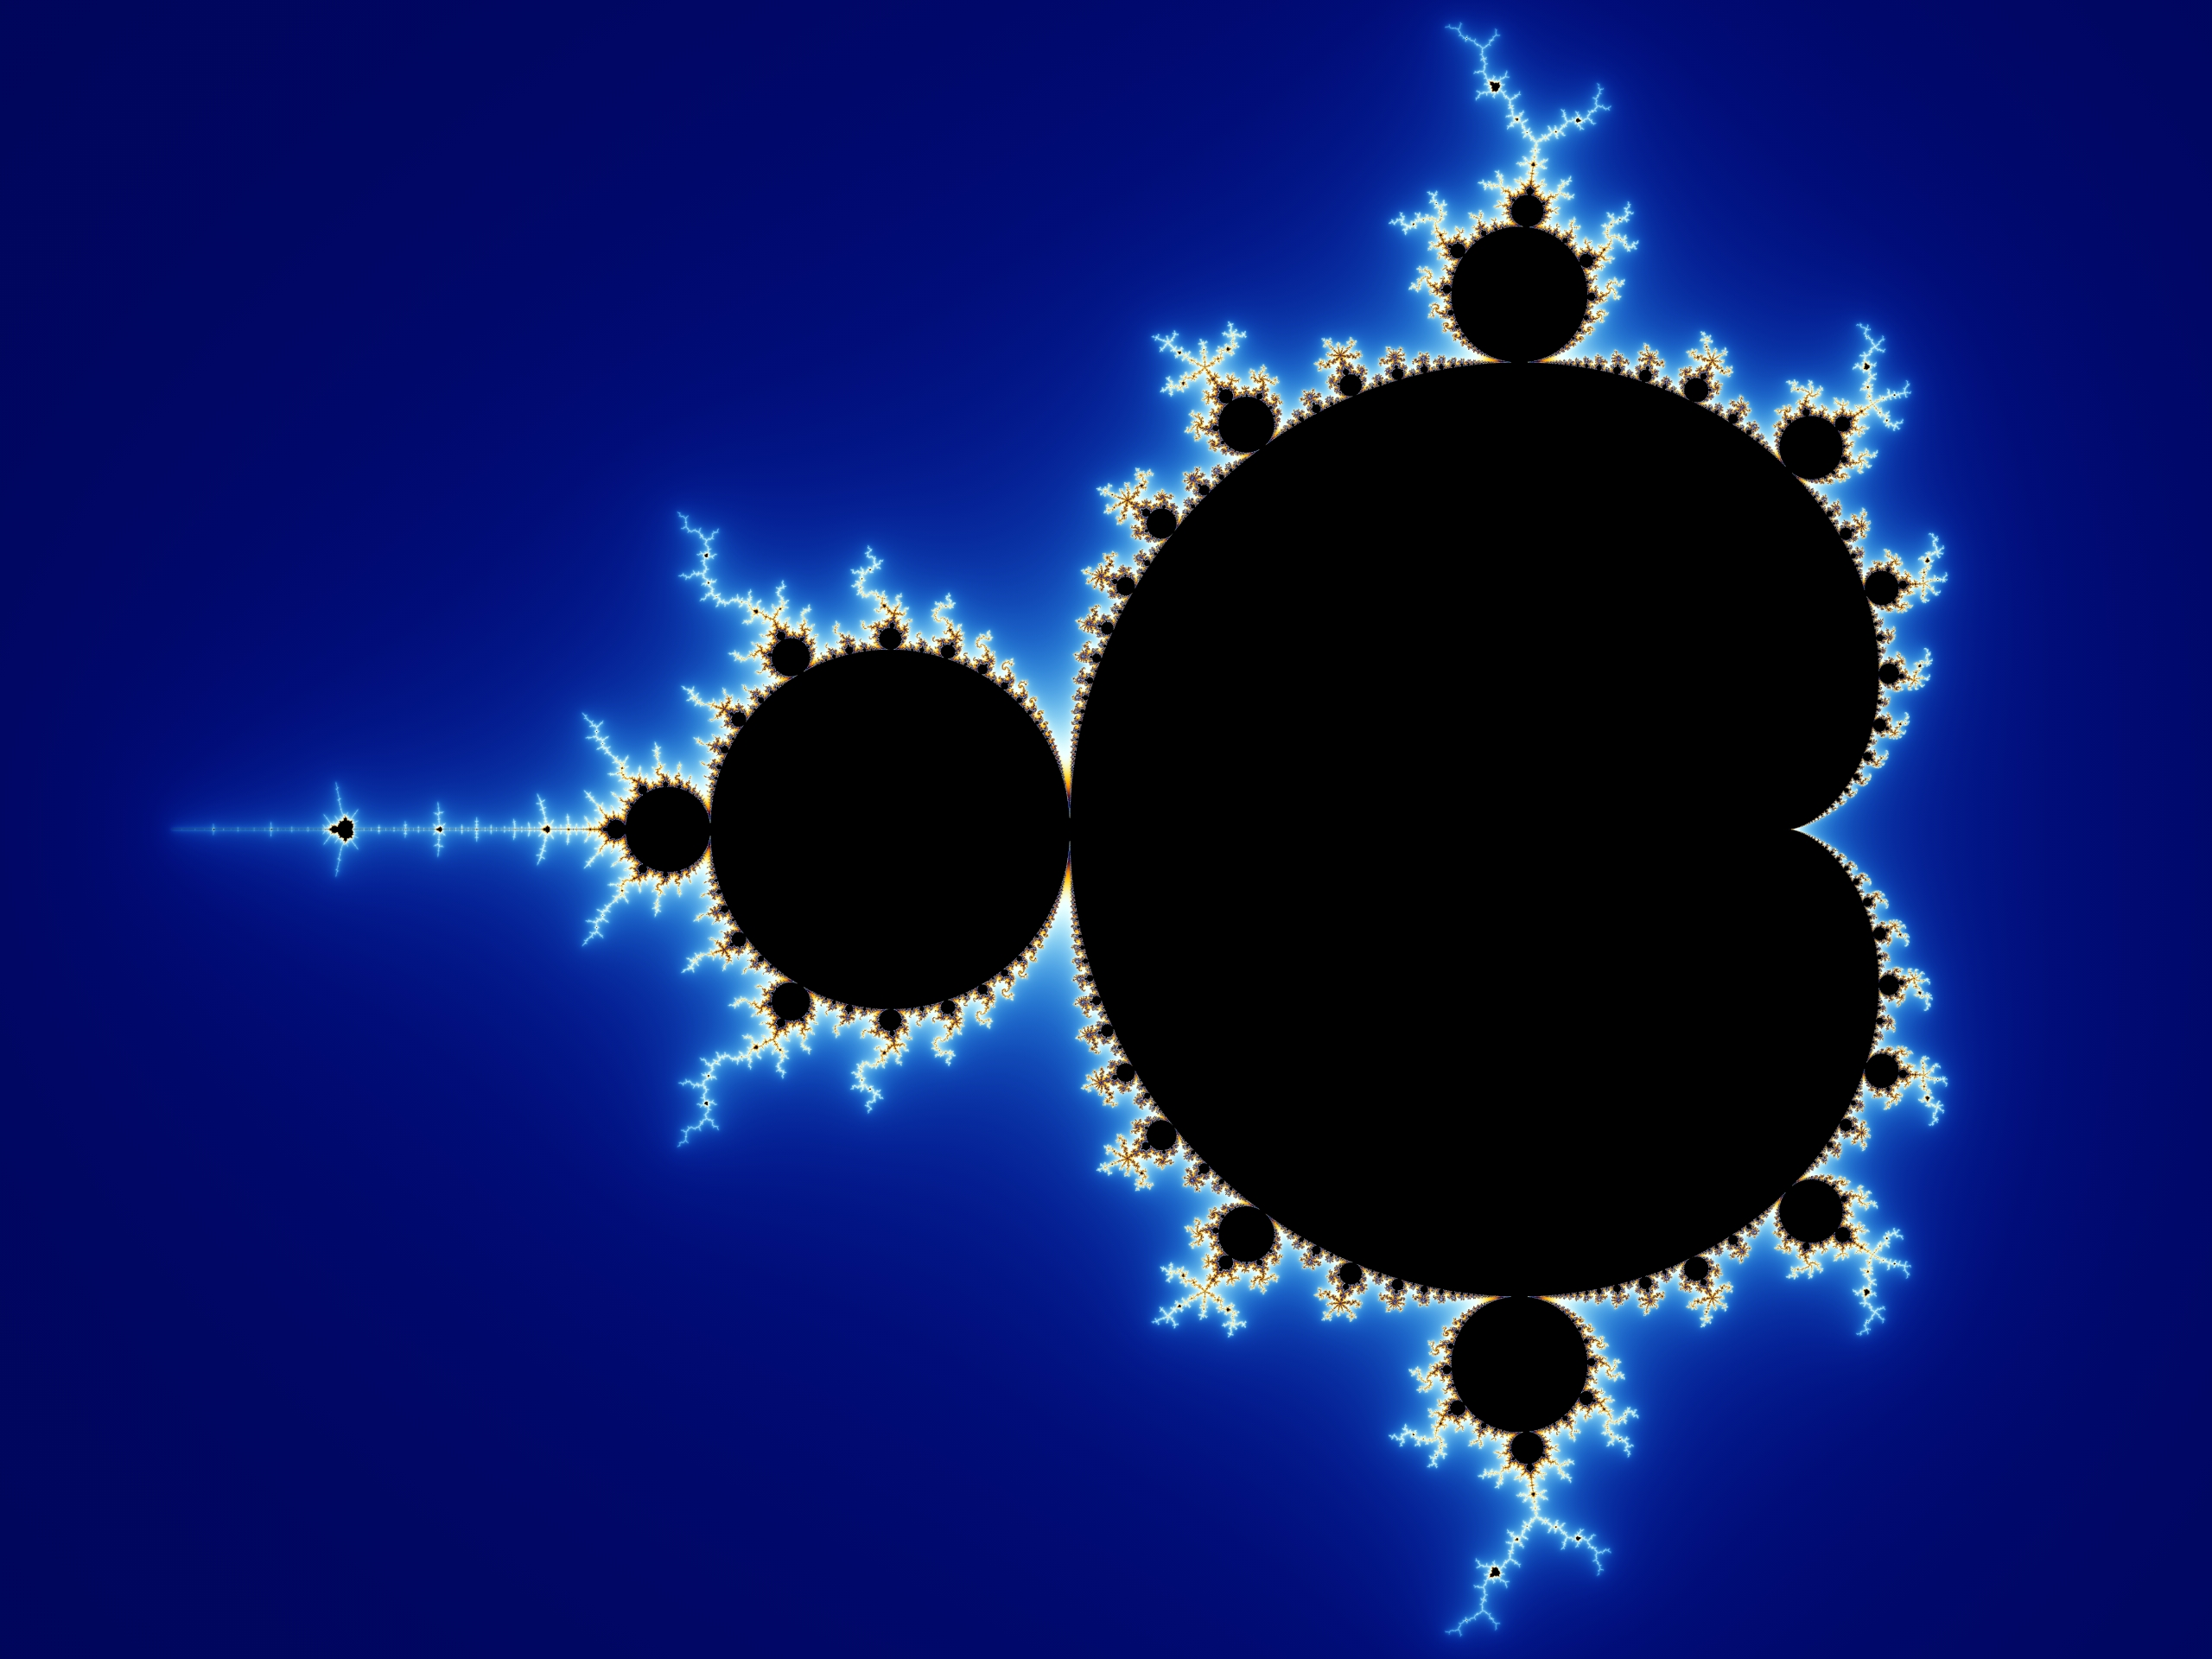
\includegraphics[width=0.8\textwidth]{images/sec-5/mandelbrot}
%     \end{center}
%     \caption[The Mandelbrot fractal]{Image of a Mandelbrot set with a
%         continuously coloured environment. Each pixel corresponds to a point $c$
%         in the complex plane, and its colour depends the number of iterations
%         $n$ before the relation diverges.}
%     \label{fig:mandelbrot}
% \end{figure}
% 
% \note{Introduce the (?) operator, talk about what divergence is, why it is bad,
% etc.}
% 
% How can we express this computation in a language without iteration? Instead, we
% use generative (meta-programming) techniques to express the recurrence relation.
% Begin by first defining a single step of the relation for a single point in the
% plane. For each point $c$ we keep a pair of elements $\left( z, n \right)$ where
% $z$ is the current value of the relation and $n$ is the iteration that
% divergence occurred at, or the current iteration otherwise.
% %
% \begin{lstlisting}[style=haskell]
% iter :: Exp Complex -> Exp (Complex, Int) -> Exp (Complex, Int)
% iter c z_n = ...
% \end{lstlisting}
% %
% This computes the next value of the polynomial $z_{n+1}$ as well as the number
% of iterations $n$ if the element has not diverged, otherwise returns the value
% and iteration count (at divergence) unchanged. We then lift this to the
% Accelerate array language by applying the operation at all points in the plane
% \code{cs}:
% %
% \begin{lstlisting}[style=haskell,firstnumber=last]
% step :: Acc (Array DIM2 (Complex,Int)) -> Acc (Array DIM2 (Complex,Int))
% step = A.zipWith iter cs
% \end{lstlisting}
% %
% Note that we have to apply the function even to elements that have already
% diverged. This wastes work but means that there is less SIMD divergence because
% we still do the same thing to every element at every iteration. Here the ``same
% thing'' does imply a small amount if divergence, between elements that have
% already diverged and those that have not, but w
% 
% We can then use
% standard Haskell to unroll the loop a \emph{fixed} number of times, which
% completes the Mandelbrot set calculation:
% %
% \begin{lstlisting}[style=haskell,firstnumber=last]
% mandelbrot :: Acc (Array DIM2 (Complex,Int)) -> Acc (Array DIM2 (Complex,Int))
% mandelbrot = foldr ($) zs0 (replicate depth step)
% \end{lstlisting}
% %
% Here \code{foldr} and \code{replicate} come from the standard Haskell
% prelude, and \code{depth} is the maximum iteration count of the relation.
% 
% This correctly computes the Mandelbrot set, but is outrageously slow because it
% must read and write the values $z$ and $n$ to memory at each step of the
% computation, rather than keeping these values in registers, computing the entire
% recurrence relation and storing only the final result to memory. Later, we will
% see how the technique of \emph{array fusion} (\S\ref{sec:fusion}) can be used to
% eliminate this intermediate memory traffic by combining the \emph{depth}
% applications of the collective operation \code{zipWith iter} into a single
% operation containing \code{depth} instances of the scalar function
% \code{iter}, which does not require us to write the intermediate values to
% memory. However, doing this we uncover an embarrassing secret: \emph{a C
% compiler does not compile C code}, it compiles \emph{idiomatic} C code. While
% combining the sequence of collective operations into a single collective
% operation containing a sequence of scalar operations produces faster code due to
% reduced memory traffic, it is still far from optimal.
% 
% The problem is that fusing the collective operations in this way does not
% preserve the iteration structure of the recurrence relation, and the loop is
% completely unrolled in the single fused operation. We can introduce scalar loops
% by looking for the following pattern:
% %
% \begin{lstlisting}[style=Haskell,numbers=none,mathescape]
% %\bf$\langle$ loop introduction $\rangle$%
%     let x =
%         let y = e1
%         in e2
%     in e3
%     $\mapsto$
%     iterate[2] (\y -> e2) e1            %\rm if \texttt{e2} $\equiv$ \texttt{e3}%
% \end{lstlisting}
% %
% The nested bindings are replaced with an explicit scalar value iteration
% structure, where the expression \code{e2} is repeated twice with the initial
% value \code{e1}. Similarly, loops can be joined:
% %
% \begin{lstlisting}[style=Haskell,numbers=none,mathescape]
% %\bf$\langle$ loop joining $\rangle$%
%     let x = iterate[n] f e1
%     in e2
%     $\mapsto$
%     iterate[n+1] f e1                   %\rm if the body of \texttt{f} $\equiv$ \texttt{e2}%
% \end{lstlisting}
% %
% Recovering scalar loops in this way enables a backend to generate explicit loops
% in its target language, such as CUDA, and ultimately results in higher
% performance code. In future, it would be beneficial to augment it with related
% loop optimisations such as loop invariant code motion in the frontend and
% lower-level code generation optimisations in a backend.


\section{The Transformations Interacting}

This section follows a few examples to discuss the effect of applying the
transformations described in the preceding sections. Many of these motivating
examples have shown up in real applications. The effects usually involve a
combination of many transformations and so give an idea of how the
transformations interact with one another.

\subsection{Ordering}

\note{TK: review}

There are several possible orderings for the transformations discussed in this
chapter, and one can easily invent examples to show that no order can be optimal
for all programs, but some orderings are generally preferable to others. This
section describes the motivation for the current sequence of transformations.

Consider the term \code{zipWith f xs xs}. The fusion transformation rewrites
this into \code{generate} style as per
section~\ref{sec:producer_producer_fusion}. Before simplification this produces
the following term, rewritten slightly: \note{TK: no, it doesn't anymore}
%
\begin{lstlisting}[style=haskell]
let a0 = use (Array ...)
    a1 = a0
    a2 = a1
    a3 = a1
in generate (intersect (shape a2) (shape a3))
            (\x0 -> let x1 = a2!x0
                        x2 = a3!x0
                    in x1 + x2)
\end{lstlisting}
%
There are a number of simplifications we would like to apply to this expression,
including shrinking (\S\ref{sec:simplification}) and common subexpression
elimination (\S\ref{sec:redundancy_elimination}). The additional array bindings
are an artefact of the way the fusion transformation handles extended
environment bindings \note{which Trevor is ashamed of and has promised to fix},
and clearly all array variables refer to the same manifest data, \code{xs} in
the expression expression. Applying shrinking to the array terms conceals this
infelicity:
%
\begin{lstlisting}[style=haskell]
let a0 = use (Array ...)
in generate (intersect (shape a0) (shape a0))
            (\x0 -> let x1 = a0!x0
                        x2 = a0!x0
                    in  x1 + x2)
\end{lstlisting}
%
Applying shrinking simplifies the binding structure making it apparent that the
scalar terms are indeed referring to the same array. If we follow the same
strategy of shrinking the scalar expressions:
%
\begin{lstlisting}[style=haskell]
let a0 = use (Array ...)
in generate (intersect (shape a0) (shape a0))
            (\x0 -> a0!x0 + a0!x0)
\end{lstlisting}
%
This term is a completely valid interpretation of the source program that does
not introduce any additional work, but we can do better. Applying shrinking
inlines the two terms \code{x1} and \code{x2} because they are each only
referenced once in the body, resulting in two accesses of the array to the same
index. Since the straightforward implementation of common subexpression
elimination is aimed at removing redundant let-bindings, we should always apply
redundancy elimination before shrinking, resulting in a term that only accesses
the underlying array once:
%
\begin{lstlisting}[style=haskell]
let a0 = use (Array ...)
in generate (intersect (shape a0) (shape a0))
            (\x0 -> let x1 = a0!x0
                    in  x1 + x1)
\end{lstlisting}

\subsection{Repeated Evaluations}
\note{TK: we only do this for scalar simplifications}

\subsection{Error tests eliminated}
\note{TK: for example: reshape, indexing}

\subsection{Confluence and Termination}

The set of transformations can be seen as a set of term rewriting rules. We
would like this set of transformations to be:
%
\begin{itemize}
    \item Correct: The transformed code retains the same semantics as the
        original code. This correctness is proved in
        section~\derp.

    \item Improving efficiency: The transformed code should require less time
        and/or fewer resources to execute than the original. We return to this
        topic in the analysis of benchmarks in chapter~\ref{ch:results}.
\end{itemize}
%
In addition, it would be of significant practical advantage if the
transformations were:
%
\begin{itemize}
    \item Confluent: When more than one transformation is applicable to a given
        term, applying the transformations in any ordering should yield the same
        result. This is important to ensure that opportunities to apply
        transformations are not lost, or worse code is generated, due to
        the choice of applying one transformation before another.

    \item Terminating: We reach a point when no transformation is applicable so
        the simplification process stops. One must be careful that one
        transformation [sequence] can not generate terms that can be transformed
        back to the original; that no transformation undoes the work of another.
\end{itemize}

\note{TK: Do some work dis/proving these two things, then write about it here.}


\section{Compiling the TK program}

\note{TK: Step through compiling a particular program, the effect each
optimisation has, needing to iterate simplifications etc. Probably need a few
different example programs.}


\section{Conclusion}

